\chapter{State of the Art and Related Research} % Main chapter title
\label{Chapter2}

\section{Energy consumption measurement and efficiency on data center level}

Energy consumption and efficiency on a data center level has been well-studied to the point where various Literature reviews were published\parencite{long2022review, jin2020review}. The bigger part of this research is focused on the data center infrasturture (cooling and power), and with good reason, as the data center infrastructure is responsible for a large part of the energy consumption. While a large number of coarse-, medium- and fine-grained metrics for data center energy consumption exist, most data center operators have focused on improving coarse-grained mertrics (especially the \textit{Power Utilization Effectiveness, PUE}) with improvements to infrastructure. This has resulted in a PUE of 1.1 or lower in some cases\parencite{uptime2023pue}. Meanwhile, server energy efficiency has substantially improved, especially for partial load and idle power\parencite{tropgen202416}. This has allowed data center operators to improve energy efficiency by simply installing more efficient cooling and power systems and servers. Fine-grained metrics such as server component utilization rates or speed were generally not used in the context of energy efficiency, but rather as performance metrics to ensure customer satisfaction.

\section{Energy consumption measurement on a server level}

As a result of the energy efficiency improvements of both data center infrastructure and server hardware mentioned in the previous section, a shift has started towards evaluating the actual server load energy efficiency. Efficiency gains on this level compound into further gains at the data center level. The method of resource-sharing of modern cloud computing (and especially the use of containers) have created great opportunities for server workload optimitation for energy efficiency, which in turn require power consumption measurements for evaluation. In the context of containers on multi-core processors, measuring the energy consumption of the entire server is insufficient, since it does not allow the attribution of consumped energy to specific containers or processes. While component-level power measurements provide finer measurements that could theoretically be modelled to display container energy consumption, they drastically raise the complexity for a number of reasons:

\begin{itemize}
    \item Component-level energy consumption measurement without external tools is far from easy. While some components provide estimation models (e.g. Intel RAPL or \textit{Nvidia Management Library} (NVML)), others can only be estimated using their performance metrics. This will invariably lead to large measurement uncertainties, especially with the component hardware differences between generations and manufacturers.
    \item The problem of attributing measured or estimated energy consumption to individual containers is in itself non-trivial: It not only requires a fine-grained time synchronization of energy consumption and used container resources due to the fast-switching nature most server components during any sort of multitasking.
    \item A deep understanding of dynamic or static energy consumption is required: Depending on the energy consumption attribution model, a container might not only account the energy it actively used, but potentially also account for a fraction of the energy consumed for any shared overhead such as shared hardware components, or system resources (such as the Kubernetes system architecure). This idea can be further extended: containers could potentially be penalized for any unused server resources, as these unused capacity still consume energy. These different attribution models lead to a larger debate about the goals of the measurements.
    \item Any server-level power models used to estimate the relation of individual component energy consumption suffers from the varity of different server configurations due to server specialization, such as Storage-, GPU-, or Memory-optimized servers.
\end{itemize}

In a systematic review cloud servers power models, Lin et al\parencite{lin2020taxonomy} categorize power collection methods into 4 categories:
\begin{table}[h]
    \tiny
    \begin{tabular}{ |p{2cm} | p{2cm} | p{2.5cm} | p{1.2cm} | p{2cm} | p{1.5cm} |} 
        \hline
        \textbf{Key} & \textbf{Value} & \textbf{Description} & \textbf{Deployment Difficulty} & \textbf{Data Granularity} & \textbf{Data Credibility}\\
        \Xhline{1.5pt}
        Based on instruments & Installation of extra devices & Bare-metal machines & Easy & Machine Level & Very high \\
        \hline
        Based on dedicated aquisition system & Specialized systems & Specified models of machines & Difficult & Machine or component-level & High \\
        \hline
        Based on software monitoring & Build-in power models & Bare-metal and virtual servers & Moderate & Machine, component, or VM level & Fair \\
        \hline
        Based on simulation & System simulation & Machine, component or VM level & Easy & Machine, component, or VM level & Low\\
        \hline
    \end{tabular}
    \caption[Comparison of power collection methods for cloud servers]{Comparison of power collection methods for cloud servers}
    \label{tab:power_collection_methods}
\end{table}

The following sections of this chapter aim to present the current state-of-the-art in the various fields of research of the problem domains listed above, focussing on different measurement approches: Direct hardware measurements, In-band measurement techniques and model-based estimation. The following sections are organized by measurement approach, foregoing organization by server component. For this reason, section~\ref{sec:component_specific_summaries} provides a brief summary of component-specific energy consumption measurement techniques.

\section{Direct Hardware Measurement}

\subsection{Instrument-based power data aquisition}

Instrument-based Data collection aquisition produces the hightest data credibility at a low granularity: These devices, installed externally (measuring the power supplied to the PDU) or internally (measuring the power flow between the PDU and motherboard) have been the source of information for a number of studies. The approach to simply measure electric power at convenient hardware locations using dedicated equipment can of course be extended to provide additional granularity: For example, Desrocher et al\parencite{desrochers2016validation} custom-created a DIMM extender custom-fitted with Hall-sensor resistors and a linux measurement utility to measure power consumed by a DIMM memory module at 1kHz sampling rate using a \textit{WattsAppPro?} power meter and a \textit{Measurment Computing USB.1208FS-Plus} data aquisition board.

This of course highlights a fundamental truth of instrument-based data collection: While it is possible to implement a measuring solution that provides high-granular and high-sampling rate power data, it is paired with an immense effort since solutions like this are not provided off-the-shelf. Unsuprisingly, this is most valuable for benchmarking or validation (Desrochers et al used their setup to validate Intel RAPL DRAM power estimations on three different systems). However, this methodology is (currently) unsuitable for deployment to data center servers due to its bad scalability and prohibitive costs. Hence, the primary role of instrument-based power data aquisiton is as a benchmarking and validation tool for research and development.

\subsection{Dedicated Aquisition systems}

\subsubsection{BMC Devices, IPMI and Redfish}
\label{sec:BMC_devices}
Some manufacturers have developed specialized power data aquisition systems for their own server products. The baseboard management controller (BMC) is a typical dedicated aquisition system usually integrated with the motherboard, usually as part of the intelligent platform management interface (IPMI)\parencite{lin2020taxonomy}. It can be connected to the system bus, sensors and a number of components to provide power and temparature information about the CPU, memory, LAN port, fan, and the BMC itself. Some comprehensive management systems such as Dell iDRAC or Lenovo xClarity have been further developed to provide high-quality, fine-grained power data due to their close interoperation between system software and underlying hardware. BMC devices on modern servers often offer IPMI- or Redfish interfaces. While these interfaces use the same physical servers, their implementation differ significantly, where Redfish generally offers higher accuracy (e.g through the use of higher-bit formats, whereas IPMI often uses 8-bit raw numbers).

In the context of container power consumption estimation, IPMI-implementations occupy an interesting role. In 2016, Kavanagh et al\parencite{kavanagh2016accuracy} found the accuracy of IMPI power data to be relatively inaccurate when compared with an external power meter, mainly due to the large measurement window size of 120 to 180 seconds and the inaccurate assessment of the idle power. They concluded that IMPI power data was still useful when a longer averaging window was used, and the initial datapoints discounted. In a later study, they suggest combining the measurements of IPMI and Intel RAPL (which they find to underestimate the power consumption) for a reasonable approximation of true measurement\parencite{kavanagh2019rapid}. Kavanagh's findings have been cited in various studies, often to negate the use of IPMI for power measurement. When used, it sometimes is chosed because it was the "simplest power metric to read"\parencite{white2020monitoring} in the context of entire data centers.

Redfish is a modern Out-of-band Management System, first released in 2015 explicitely to replace IPMI \parencite{thomas-krenn-redfish}. It uses a RESTful API and JSON data format, making queries with code easier. In 2019, Wang et al\parencite{wang2019empirical} directly compared IPMI and redfish power data to a reading of a high accuracy power analyzer, and found Redfish to be more accurate than IPMI, with a MAPE of 2.9\%, while also finding a measurement latency of about 200ms. They also found measurements to be more accurate in higher power ranges, which they attribute to the improved latency.

In conclusion, BMC power data aquired over Redfish provides a simple simple and comparatively easy way to measure system power based on various physical system sensors. Its biggest strenght lies in easy implementation and general availability. In the context of container energy consumption, BMC power data lacks the short sampling rates necessary to measure a a highly dynamcic container setup, but can prove useful as a validation or cross-reference dataset for longer intervals exceeding 120 seconds. Unfortunately, the data quality of BMC power data depends on the actual system, and power models can be significantly improved by initial calibration with an external power measurement device\parencite{kavanagh2016accuracy}.

\section{In-Band Measurement Techniques}

In-band measurement techniques refer to methods of power consumption monitoring that utilize built-in telemetry capabilities of system components to collect energy usage data directly from within the host system. Unlike external power meters or BMCs like IPMI, which operate independently of the main system, in-band techniques leverage on-die sensors and software interfaces to gather power metrics in real-time. These techniques provide fine-grained data with minimal additional hardware, making them well-suited for scalable environments like Kubernetes clusters. However, their accuracy and granularity are often dependent on the hardware's internal estimation algorithms, which may introduce uncertainties compared to direct measurement methods.

\subsection{ACPI}

The \textit{Advanced Configuration and Power Interface (ACPI)} is a standardized interface that facilitates power management and hardware configuration by allowing the operating system to control hardware states such as processor sleep, throttling, and performance modes \cite{uefi_acpi_6_6}. It plays a significant role in processor performance tuning by exposing C-states (idle), P-states (performance), and T-states (throttling) which the OS can leverage to adjust the processor's activity, frequency, and voltage.

Although ACPI defines these power states, their actual implementation is processor-specific, and the interface does not provide real-time telemetry. As such, ACPI does not expose instantaneous power consumption values. Any attempt to estimate power based on ACPI would require detailed knowledge of processor-specific behavior, including the mapping between frequency, voltage, and power—information that is not exposed through ACPI. As a result, limited research was conducted on this topic.

In theory, one could attempt to use ACPI's \texttt{\_PSS} (Performance Supported States) table, which lists available P-states along with nominal voltage, frequency, and optionally estimated maximum power dissipation, to perform rough CPU power estimation. This method would involve tracking CPU residency in each performance state and applying simple integration models to estimate total energy. However, due to the static nature of \texttt{\_PSS} entries and the lack of temporal precision, such estimates would be inherently coarse-grained and typically inaccurate for modern processors with dynamic voltage and frequency scaling or turbo modes.

Consequently, ACPI is rarely used in contemporary power estimation contexts. Its primary role remains in system configuration and power state control rather than accurate energy quantification. In modern Intel processors, the Running Average Power Limit (RAPL) interface provides a more appropriate solution for in-band power measurement. This makes RAPL the preferred tool for energy-aware computing research and production environments alike.

\subsection{Intel RAPL}
\label{sec:RAPL}
Intel Running Average Power Level (RAPL) is a Power Monitoring Counter (PMC)-based feature introduced by Intel and provides a way to monitor and control the energy consumption of various components within their processor package\parencite{projectexigence_rapl}. An adaptation of RAPL for AMD processors uses largely the same mechansms and the same interface\parencite{amd_energy}, although it provides less information than Intel's RAPL, providing no DRAM energy consumption\parencite{schone2021energy}. Unfortunately RAPL does not have a detailed low-level implementation documentation, and the exact methodology of the RAPL calculations remain unknown\parencite{jay2023experimental}.

Intel RAPL has been used extensively in research to measure energy consumption\parencite{kennes2023measuring} despite some objections about its accuracy, which will be discussed sections~\ref{sec:raplvalidation} and ~\ref{sec:rapllimitations}. The general concencus is that RAPL is \textit{good enough} for most scientific work in the field of server energy consumption and efficiency. As Raffin et at\parencite{raffin2024dissecting} point out, it is mostly used \textit{like a black box without deep knowledge of its behavior}, resulting in implementation mistakes. For this reason, the next section~\ref{sec:raplmethodology} presents an overview of the RAPL fundamentals.Finally, section~\ref{sec:rapltools} discusses the currently available RAPL-based tools.

\subsubsection{RAPL measurement methods}
\label{sec:raplmethodology}
This subsection provides an overview of how RAPL works and is used. It is based on the Intel rchitectures Software Developer’s Manual\parencite[Section 16.10]{intel-sdm} and the works of Raffin et al \parencite{raffin2024dissecting} (2024) and Schöne et al \parencite{schone2024energy} (2024).

Running Average Power Limit (RAPL) is a power management interface in Intel CPUs. Apart from power limiting and thermal management, it also allows to measure the energy consumed by various components (or \textit{domains}). These domains individual CPU cores, integrated graphics (in non-server CPUs) and DRAM, as well as \textit{package}, refering to the whole CPU die. While it initially used models to estimate energy use\parencite{hackenberg2015energy}, it now uses physical measurements. The processor is divided into different power domains or "planes", representing specific components, seen in figure~\ref{fig:rapl_domains}. Notably, not all domains are present in all systems: Both client-grade systems feature the \textit{Package} and \textit{PP0 core} domains, server grade processors typically don't show the \textit{PP1 uncore}-domain typically used for integrated GPUs, and client-grade processors don't show the \textit{DRAM} domain. The \textit{PSYS} domain for the "whole machine" is ill defined and only exists on client-grade systems. In an experiment with recent Lenovo and Alienware laptops, Raffin et al found that the \textit{PSYS} domain reported the total consumption of the laptop, including display, dedicated GPU and other domains. Regardless, this thesis will focus on the RAPL power domains available to server-grade processors.

\begin{figure}[ht]
    \centering
    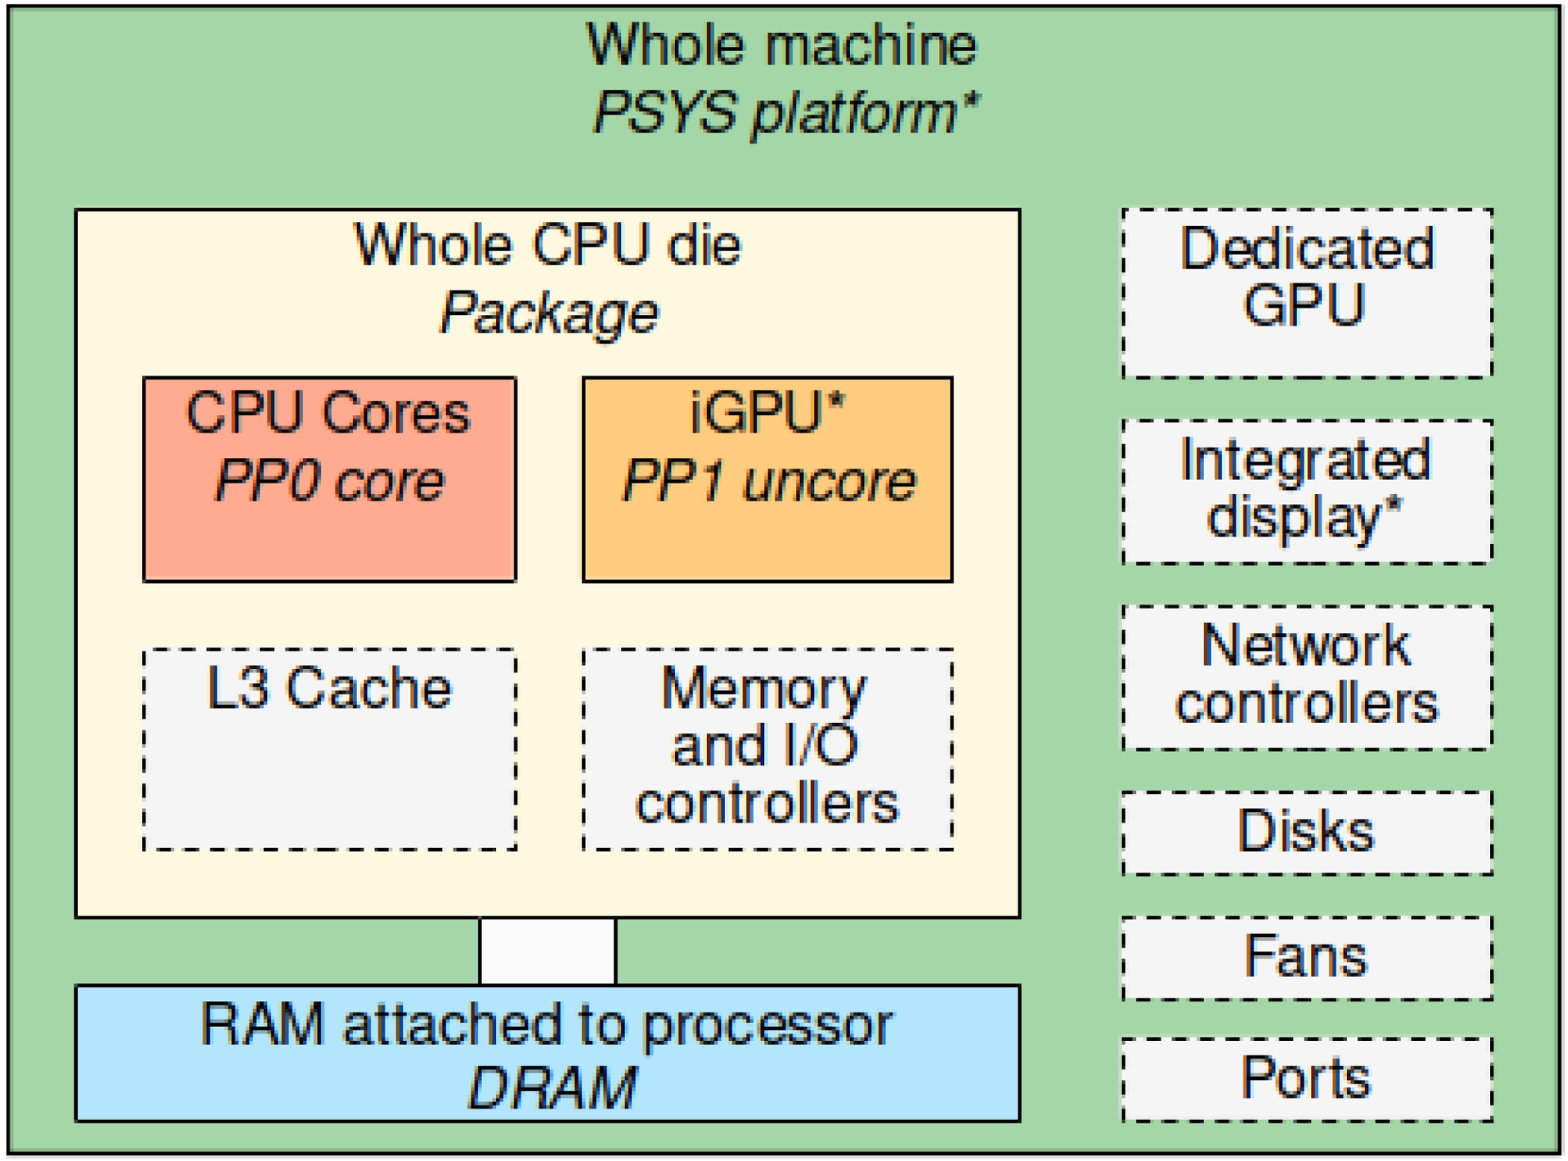
\includegraphics[width=0.7\textwidth]{Figures/rapl_domains.png}
    %\decoRule
    \caption[Rapl domains]{Hierarchy of possible RAPL domains and their corresponding hardware components. Domain names are in italic, and grayed items do not form a domain on their own, items with an asterisk are not present on servers\parencite{raffin2024dissecting}.}
    \label{fig:rapl_domains}
\end{figure}

RAPL provides hardware counters to read the energy consumption (and set power limits) for each domain. The energy consumption is measured in terms of processor-specific "energy units" (e.g. 61$\mu$J for Haswell and Skylake processors). The counters are exposed to the operating system through model-specific registers (MSRs) and are updated approximately every millisecond. The main advantages of RAPL are that no external powermeters are required, nor a privileged access to the BMC (which could be used to power off the server). RAPL is more accurate than any untuned statistical estimation model.

Various measurement methods can be used to extract RAPL measurements. In a detailed comparison, Raffin et al\parencite{raffin2024dissecting} outline their individual features and tradeoffs, which are summarize in figure~\ref{fig:rapl_interfaces_tradeoffs}:
\begin{itemize}
    \item \textbf{Lacking documentation: } Since there is no publicly available documentation of the low-level RAPL implementation, implementations are bound to suffer inaccuracies and inconsistencies due to a lack of understanding.
    \item The \textbf{Model-Specific Register (MSR)} interface provides low-level access to RAPL energy counters but is complex and hardware-dependent. Developers must manually determine register offsets and unit conversions based on processor model and vendor documentation. This method lacks safeguards, requires deep processor knowledge, and is error-prone, with incorrect readings difficult to detect. Although read-only access poses no risk to system stability, MSRs expose sensitive data and are thus restricted to privileged users (e.g., \texttt{root} or \texttt{CAP\_SYS\_RAWIO}). Fine-grained access control is not supported natively, though the \texttt{msr-safe} module offers limited mitigation.
    \item The \textbf{Power Capping (powercap)} framework is a high-level Linux kernel interface that exposes RAPL energy data through the sysfs filesystem, making it accessible from userspace. It simplifies energy measurements by automatically handling unit conversions and domain discovery, requiring minimal hardware knowledge. Though domain hierarchy can be confusing (especially with DRAM domains appearing nested under the package domain) powercap remains user-friendly and scriptable. It supports fine-grained access control via file permissions and offers good adaptability to hardware changes, provided the measurement tool doesn't rely on hard-coded domain structures.
    \item The \textbf{perf-events} subsystem provides a higher-level Linux interface for accessing RAPL energy counters as counting events. It supports overflow correction and requires less hardware-specific knowledge than MSR. Each RAPL domain must be opened per CPU socket using \texttt{perf\_event\_open}, and values are polled from userspace. While it lacks a hierarchical structure like powercap and may be harder to use in certain languages or scripts, it remains adaptable and robust across different architectures. Fine-grained access control is possible via kernel capabilities or \texttt{perf\_event\_paranoid} settings. 
    \item \textbf{eBPF} enables running custom programs in the Linux kernel, and in this context, it is used to directly read RAPL energy counters from within kernel space, potentially reducing measurement overhead by avoiding user-kernel context switches. The implementation attaches an eBPF program to a CPU clock event, using \texttt{perf\_event\_open} to access energy counters and buffering results for userspace polling (is visualized in figure~\ref{fig:rapl_perf_eBPF}).While offering the same overflow protection as regular \texttt{perf-events}, this approach is significantly more complex, prone to low-level errors (especially in C), and requires elevated privileges (\texttt{CAP\_BPF} or \texttt{root}). It also lacks portability, as it demands manual adaptation to kernel features and domain counts, limiting its maintainability across systems.
\end{itemize}
\begin{figure}[H]
    \centering
    \begin{subfigure}{0.48\textwidth}
        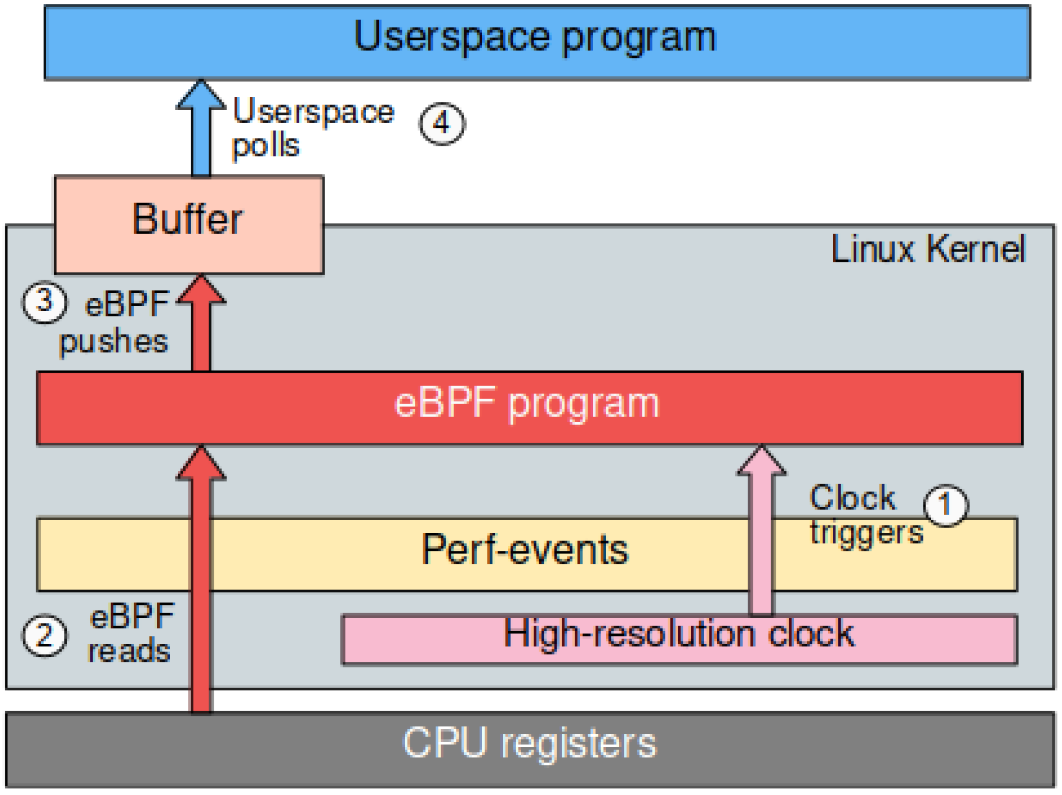
\includegraphics[width=\textwidth]{Figures/rapl_perf_eBPF.png}
        \caption[RAPL perf-event eBPF mechanism]{RAPL perf-event eBPF mechanism}
        \label{fig:rapl_perf_eBPF}
    \end{subfigure}
    \hfill
    \begin{subfigure}{0.48\textwidth}
        \vspace{1.5em}
        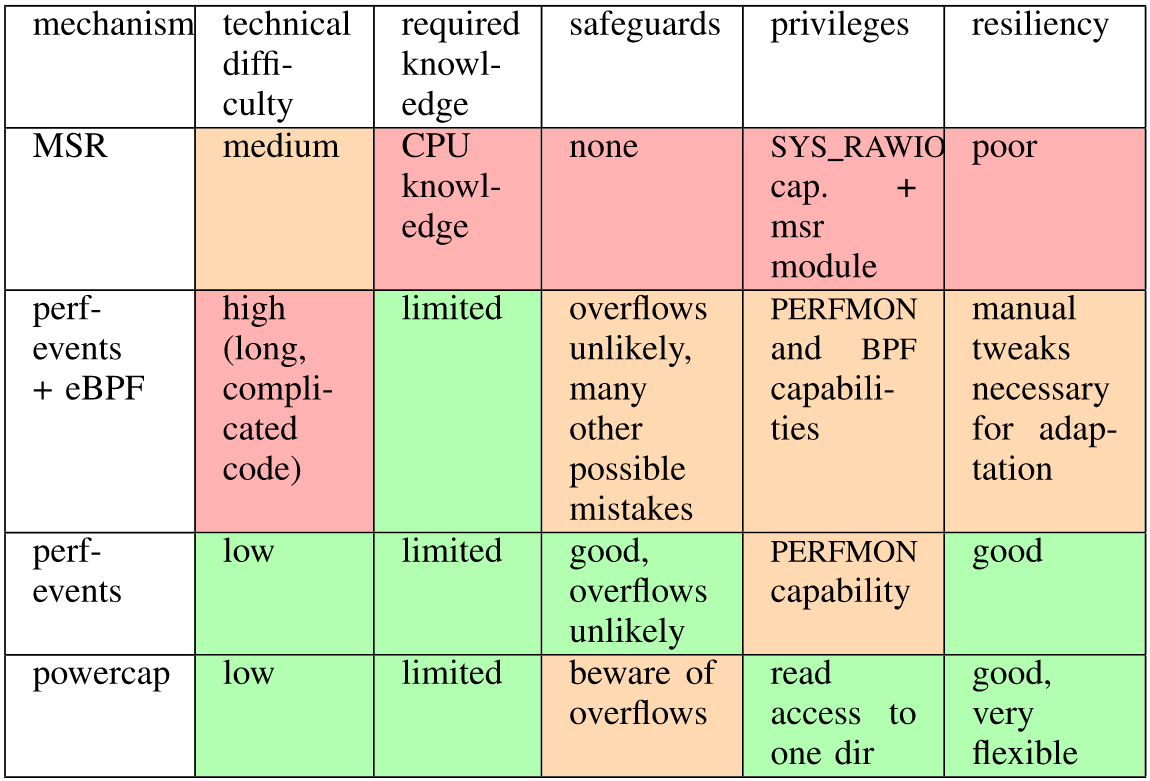
\includegraphics[width=\textwidth]{Figures/rapl_interfaces_tradeoffs.png}
        \caption[RAPL measurement mechanisms comparison]{RAPL measurement mechanisms comparison}
        \label{fig:rapl_interfaces_tradeoffs}
    \end{subfigure}
    \caption[RAPL measurements: eBPF and comparison]{RAPL measurements: eBPF and comparison\parencite{raffin2024dissecting}}
    \label{tab:measurement_mechanisms}
\end{figure}
In their research, Raffin et al conclude that all four mechanisms have small or negligible impact on the running time of their benchmarks. They formulate the following recommendations for future energy monitoring implementations:
\begin{itemize}
    \item Measuring frequencies should be adapted to the state of the node, preventing high measurement overhead, due to a reduction in time spent in low-power states. Under heavy load, a highfrequencay can be used in order to capture more information.
    \item \texttt{perf-events} is the overall recommeded measurement method with good efficiency, latency and overflow protection. Powercap is less efficient, but provides a simpler sysfs API.
    \item Even though \texttt{perf-events} and eBPF-measurement method seems to be the most energy-efficient, it is not recommended in light of its complexity. For the same reason, the MSR method is not recommeded, as it raises complexity while counter-intuitively being slower than \texttt{perf-events}
\end{itemize}

RAPL MSRs can be read on some cloud computing resources (e.g. some Amazon EC2-instances), although the hypervisor traps the MSR reads, which can add to the polling delay. in EC2, the performance overhead also significantly increases to <2.5\% (as compared to <1\% on standalone systems)\parencite{jay2023experimental}.

\subsubsection{RAPL Validation}
\label{sec:raplvalidation}
Since its inception, RAPL has been subject of various validation studies, with the general concensus that it's accuracy could be considered "good enough"\parencite{raffin2024dissecting}. Notable works are Hackenberg et al, that in 2013 found RAPL accurate but missing timestamps\parencite{hackenberg2013power}, and in 2015 noticed a major improvement to RAPL accuracy, after Intel switched from a modeling approach to actual measurements for their Haswell architecture\parencite{hackenberg2015energy}. Desrochers et al concluded in a 2016 RAPL DRAM validation study\parencite{desrochers2016validation} that DRAM power measurement was reasonably accurate, especially on server-grade CPUs. They also found measurement quality to drop when measuring and idling system. Later, Alt et al\parencite{alt2024experimental} tested DRAM accuracy of heterogeneous memory systems of the more recent Ice Lake-SP architecture and concluded that DRAM estimates behaved differently than on older architectures. They noted that the RAPL overestimates DRAM energy consumption by a constant offset, which they attribute to the off-DIMM voltage regulators of the memory system.

A critical point in the RAPL validation was the introduction of the Alder Lake architecture, marking Intel's first heterogeneous processor, combining two different core architectures from the Core and Atom families (commonly referred to as P-Cores and E-cores) to improve performance and energy efficiency. While this heterogenity can improve performance and energy efficiency, it also increases complexity of scheduling decisions and power saving mechanisms, adding to the already complex architecture, featuring per-core Dynamic Voltage and frequency Scaling (DVFS), Idle states and Power Limiting / Thermal Protection.

Schöne et al\parencite{schone2024energy} found RAPL in the Alder Lake architecture to be generally consistent with external measurements, but exhibiting lower accuracy in low power scenarios. The following figure~\ref{fig:rapl_vs_PSU_validation} shows these inaccuracies, albeit tested on a conusmer-grade Intel Core i9-12900K processor measured at the base frequency of 0.8GHz.
\begin{figure}[ht]
    \centering
    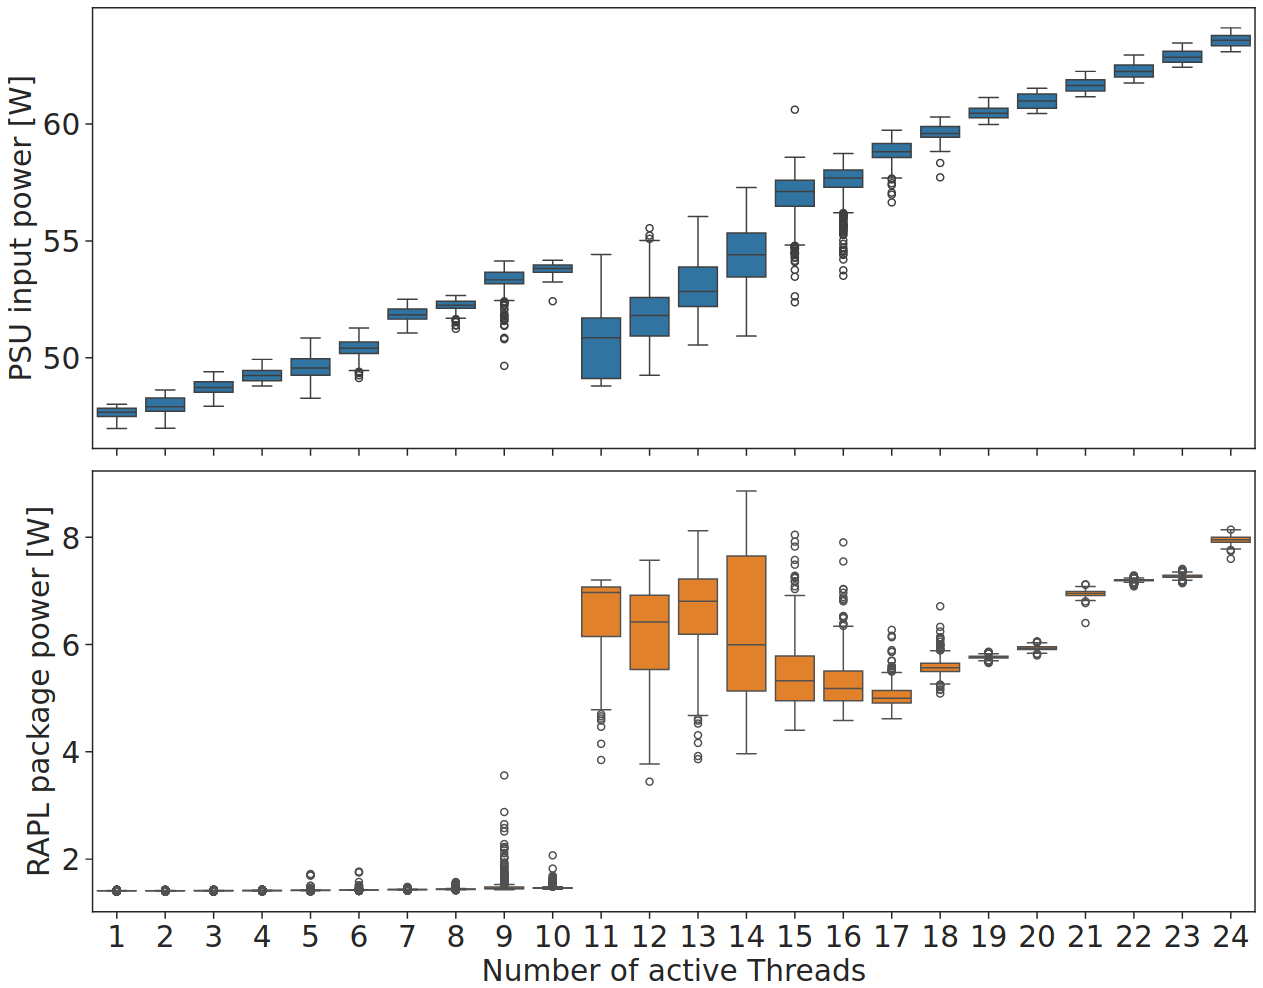
\includegraphics[width=0.7\textwidth]{Figures/rapl_vs_PSU_validation.png}
    %\decoRule
    \caption[RAPL validation: CPU vs. PSU]{RAPL and reference power consumption sampled at 100 ms / 50 ms intervals respectively. Double precision matrix multiplication kernel at 0.8GHz running for 60s each at increasing number of active threads\parencite{schone2024energy}.}
    \label{fig:rapl_vs_PSU_validation}
\end{figure}

\subsubsection{RAPL Limitations and issues}
\label{sec:rapllimitations}
Several limitations of RAPL were noticed in various research works. Since RAPL is continually improved by Intel as new Processors are released, some of these issues have since been improved or entirely solved. 

\begin{itemize}
    \item \textbf{Register overflow: }The 32-bit register can experience an overflow error\parencite{khan2018rapl, raffin2024dissecting}. This can be mitigated by sampling more frequently than the register takes to overflow. This interval can be calculated using the following equation: 
    \begin{equation}
        t_{\text{overflow}} = \frac{2^{32} \cdot E_u}{P}
    \end{equation}
    Here, $E_u$ is the energy unit used (61$\mu$J for haswell), and $P$ is the power consumption. On a Haswell processor consuming 84W, an overflow would occur every 52 minutes. Intel acknowledges this in the official documentation, stating that the register has a \textit{wraparound time of around 60 seconds when power consumption is high}\parencite{intel-sdm}
    This is solvable with a simple correction, provided that the measurement interfals are small enough: For two successive measurements $m_{\text{prev}}$ and $m_{\text{current}}$, the actual measured difference is given by
    \begin{equation}
        \Delta m =
        \begin{cases}
        m_{\text{current}} - m_{\text{prev}} + C & \text{if } m_{\text{current}} < m_{\text{prev}} \\
        m_{\text{current}} - m_{\text{prev}} & \text{otherwise}
        \end{cases}
    \end{equation}
    where C is a correction constant that depends on the chosen mechanism:
    
    \begin{table}[h]
        \small
        \begin{tabular}{|p{4cm}|p{9cm}|}
            \hline
            \textbf{mechanism} & \textbf{constant C}\\
            \Xhline{1.5pt}
            MSR & \texttt{u32::MAX} i.e. $2^{32} - 1$\\
            \hline
            perf-events & \texttt{u64::MAX} i.e. $2^{64} - 1$\\
            \hline
            perf-events with eBPF & \texttt{u64::MAX} i.e. $2^{64} - 1$\\
            \hline
            powercap & value give by the file \texttt{max\_energy\_uj} in the sysfs folder for the RAPL domain\\
            \hline
        \end{tabular}
        \caption[RAPL overflow correction constant]{RAPL overflow correction constant}
        \label{tab:RAPL_overflow_correction_constant}
    \end{table}

    \item \textbf{DRAM Accuracy: }DRAM Accuracy can only reliably be used for the Haswell architecture\parencite{desrochers2016validation, khan2018rapl, alt2024experimental}, and may still exibit a constant power offset (like attributed to the voltage regulator power loss of the memory system).
    \item \textbf{Unpredictable Timings: }While the Intel documentation states that the RAPL time unit is 0.976ms, the actual intervals may vary. This is an issue since the measurements do not come with timestamps, making precise measurements difficult\parencite{khan2018rapl}. Several coping mechanisms have been used to mitigate this, notably \textit{busypolling} (busypolling the counter for updates, significantly compromizing overhead in terms of time and energy\parencite{hahnel2012measuring}), \textit{supersampling} (lowering the sampling interval, increasing overhead and occasionaly creating duplicates that need to be filtered\parencite{khan2018rapl}), or \textit{high frequency sampling} (\textit{lowering} the sampling rate when the resulting data is still sufficient\parencite{servat2016detailed}). Another solution is to use a \textit{low sampling frequency} to smoothe out the relative error due to spikes, with the only drawback of loss of temporal precision. At sampling rates slower than 50Hz, the relative error is less than 0.5\% \parencite{jay2023experimental}.
    \item \textbf{Non-atomic register updates: } RAPL register updates are nont atomic\parencite{khan2018rapl}, meaning that the different RAPL values show a delay between individual updates. This may introduce errors when sampling multiple counters at a high sampling rate, making it possible to read both fresh and stale values of different counters.
    \item \textbf{Lower idle power accuracy: } When measuring an idling server, RAPL tends to be less accurate\parencite{schone2024energy, desrochers2016validation}.
    \item \textbf{Side-channel attacks: } While the update rate of RAPL is usually 1ms, it can get as low as 50 $\mu$s for the PP0 domain (processor cores) on desktop processors\parencite{schone2024energy}. This can be used to retrieve processed data in a side channel attack (coined "Platypus")\parencite{lipp2021platypus, schone2024energy}. 
    
    To mitigate this issue while retaining RAPL functionality, Intel implements a filtering technique via the \texttt{ENERGY\_FILTERING\_ENABLE}\parencite[Table 2-2]{intel2023} entry, or when \textit{Software Guard Extension (SGX)} is activated in the BIOS. This filter adds random noise to the reported values (vizualized in Figure~\ref{fig:rapl_platypus_filtering}). This can be seen For the PP0 domain, this raises the temporal granularity to about 8ms. While this does not affect the average power consumption, point measurement power consumption can be affected. Figure~\ref{fig:rapl_filter_granularity_loss} shows the effect of the filter, clearly indicating the loss granularity resulting from the activation of the filter. In a 2022 article, Tamara\parencite{greencoding_rapl_sgx} found a surprising higher mean with the filter activated and deemed filtered RAPL energy data unusable. In a more elaborate experiment in 2024, Schöne et al did not encounter these inaccuracies anymore.

    \begin{figure}[H]
        \centering
        \begin{subfigure}[t]{0.6\textwidth}
            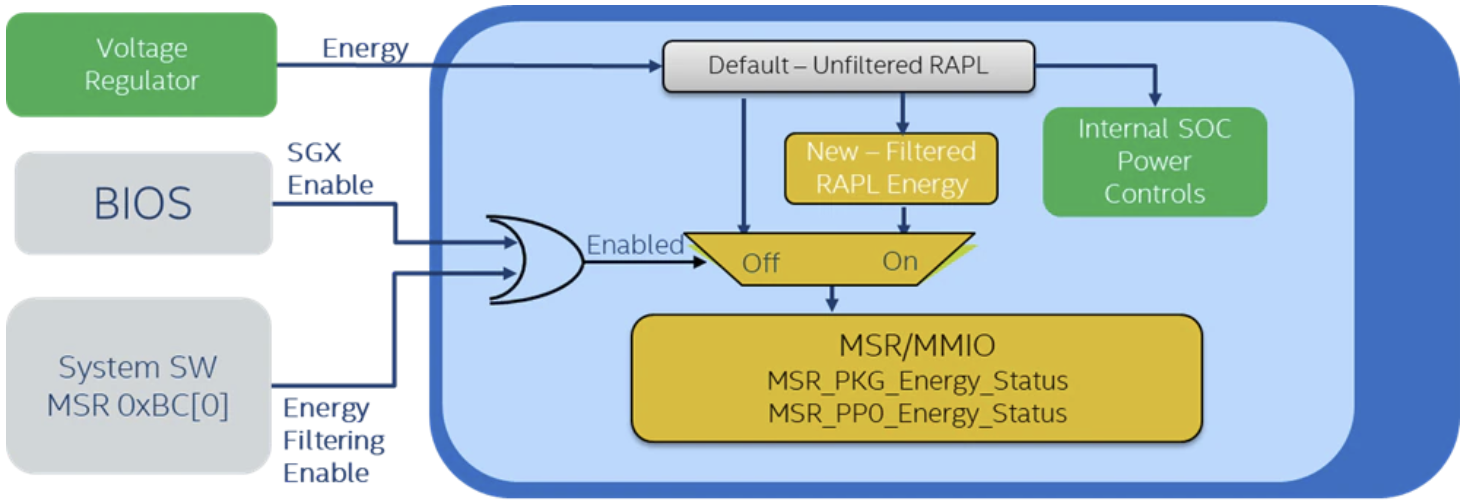
\includegraphics[width=\textwidth]{Figures/rapl_platypus_filtering.png}
            \caption{RAPL energy filtering\parencite{intel_rapl_guidance}}
            \label{fig:rapl_platypus_filtering}
        \end{subfigure}
        \begin{subfigure}[t]{0.48\textwidth}
            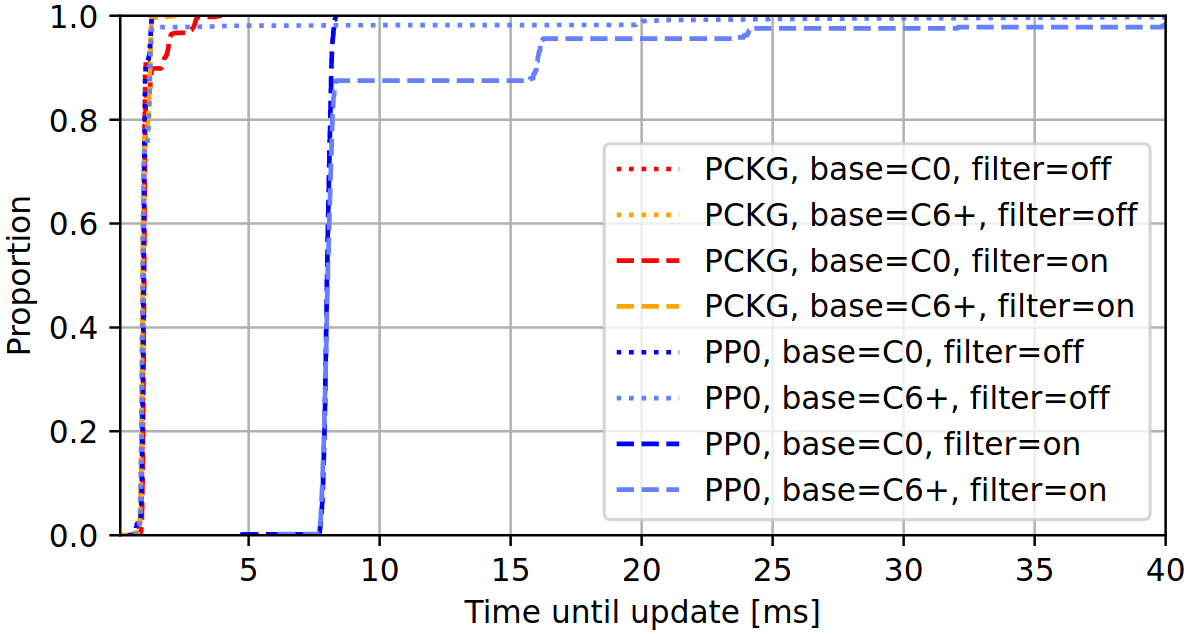
\includegraphics[width=\textwidth]{Figures/rapl_filter_granularity_loss_time.png}
            \caption{Distribution of time between updates: With an enabled filter, the PP0 domain only provides updates every 8 ms, otherwise RAPL values are updated every 1 ms. If the load is too low, some updates might be skipped, e.g., the next update for PP0 and an enabled filter is at 16 ms.}
            \label{fig:rapl_filter_granularity_loss_time}
        \end{subfigure}
        \hfill
        \begin{subfigure}[t]{0.48\textwidth}
            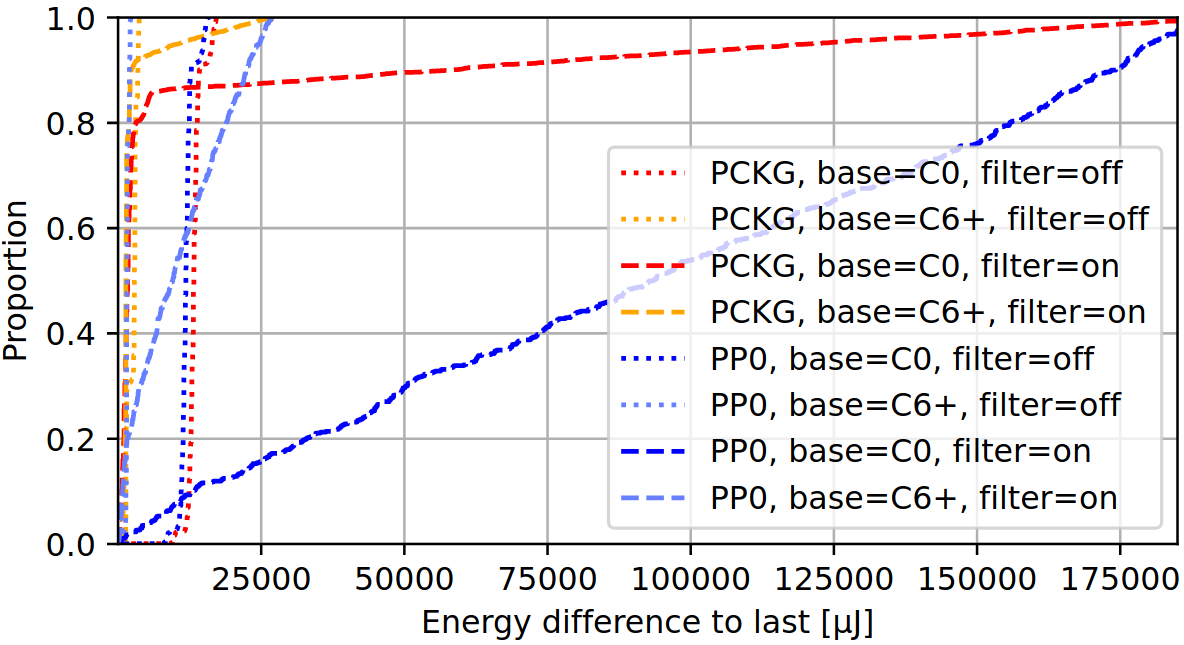
\includegraphics[width=\textwidth]{Figures/rapl_filter_granularity_loss_energy.png}
            \caption{The minimal increase of a measurement is 1 energy unit of 61.035~$\mu$J. Enabling the filter leads to a significant influence on measurements for the PP0 domain and a measurable influence on PCKG measurements.}
            \label{fig:rapl_filter_granularity_loss_energy}
        \end{subfigure}
        \caption[RAPL \texttt{ENERGY\_FILTERING\_ENABLE Granularity loss}]{Observable loss of granularity caused by the activation of \texttt{ENERGY\_FILTERING\_ENABLE}\parencite{schone2024energy}}
        \label{fig:rapl_filter_granularity_loss}
    \end{figure}
\end{itemize}

\subsubsection{RAPL conclusions}

The energy measurement accuracy of RAPl has significantly improved since its inception and provides a generally accepted way to measure system energy consumption. It is well-validated and accepted as the most accurate fine-granular energy measurement tool. Some known limitations have historically created inaccuracies in developed measurement tools, but corrections of these limitations exist. 

\subsection{Graphical Processing Units (GPU)}
In recent years, the utilization of GPUs in cloud computing environments has grown significantly, driven primarily by the increasing demand for high-performance computations in machine learning, artificial intelligence, and large-scale data processing \cite{jouppi2017datacenter}. Kubernetes now includes mechanisms for GPU provisioning, enabling containerized workloads to leverage GPU acceleration \cite{k8s_gpu_support}.

Although GPUs remain less common than traditional CPU-based workloads in typical Kubernetes clusters, their adoption is rapidly accelerating. Industry reports indicate that GPU usage in Kubernetes has seen a growth rate of nearly 58\% year-over-year, outpacing general cloud computing growth rates \cite{datadog_report}. This increase is largely attributed to ML workloads and real-time processing tasks that benefit from the parallel processing capabilities of GPUs \cite{tensorflow_k8s}. Furthermore, hyperscalers have integrated GPU support directly into their managed Kubernetes services, reflecting the growing demand for GPU-powered workloads in containerized environments.

Despite this growth, GPU deployments are still not as pervasive as CPU-based workloads in Kubernetes-managed clusters. The primary focus of this thesis is on the measurement and analysis of energy consumption in more common, CPU- and memory-centric Kubernetes workloads. Nevertheless, due to the rising significance of GPUs, their energy measurement techniques and potential integration within Kubernetes environments are briefly examined.

Ultimately, the inclusion of GPU energy measurements remains outside the primary scope of this thesis but is acknowledged as an important area for future research. This structured exploration serves to highlight current limitations and opportunities for enhancing energy efficiency in Kubernetes-managed GPU workloads.

\subsubsection{GPU virtualization technologies}

\paragraph{Full GPU Virtualization}

Full GPU virtualization provides isolated instances of a single physical GPU to multiple virtual machines. This is achieved using technologies such as NVIDIA's \textit{vGPU} or AMD's \textit{MxGPU (Multiuser GPU)}. These technologies allow a VM to see a complete GPU, while the underlying hypervisor manages resource partitioning and scheduling \cite{nvidia_virtualization, amd_instinct_virtualization} eigher though the use of partitioning or time-slicing. In a Kubernetes environment, full GPU virtualization is commonly utilized through:
\begin{itemize}
    \item \textbf{vGPU on VMware or OpenStack:} Kubernetes clusters running on VMware vSphere or OpenStack can request vGPU instances as if they were physical GPUs. These instances are shared among containers while maintaining memory and compute isolation.
    \item \textbf{Device Plugin Integration:} NVIDIA, AMD and Intel provide a Device Plugin for Kubernetes, enabling seamless GPU discovery and allocation across pods \cite{k8s_gpu_support}.
\end{itemize}

\paragraph{Multi-Instance GPU (MIG)}
Introduced with the NVIDIA A100 architecture, Multi-Instance GPU (MIG) allows a single GPU to be partitioned into up to seven independent instances, each with its own dedicated compute, memory, and cache resources \cite{nvidia_mig_user_guide}. Unlike traditional vGPU, MIG provides true hardware-level isolation, preventing noisy-neighbor effects and enabling finer resource allocation. MIG instances are exposed to Kubernetes as individual GPUs. For example, a single A100 GPU partitioned into seven MIG instances appears as seven separate GPU resources, each assignable to different containers. MIG-aware device plugins ensure proper scheduling and isolation. Hence, MIG technology is particularly useful for multi-tenant environments and supports finer granularity in resource allocation compared to traditional vGPU models.

\paragraph{GPU Passthrough}
GPU passthrough allows a physical GPU to be exclusively assigned to a single VM or container. Unlike virtualization, where resources are shared, passthrough dedicates the full GPU to one environment, offering near-native performance \cite{nvidia_passthrough}. GPU passthrough is configured at the hypervisor level (e.g., KVM or VMware ESXi) and can be exposed to Kubernetes nodes. Pods scheduled on nodes with GPU passthrough access gain complete control of the GPU, enabling direct memory access and high-performance computation.

GPU virtualization technologies enable efficient multi-tenant use of GPU resources, enhancing performance and cost-effectiveness in cloud-native environments. For the purposes of energy measurement, understanding these virtualization layers is essential for accurate per-container energy attribution.

\subsubsection{GPU nvidia-NVML energy measurements and validation}

Modern GPUs are equipped with \textbf{built-in power sensors} that enable real-time energy measurement. For instance, Nvidia GPUs expose power metrics through the \textit{Nvidia System Management Interface (nvidia-smi)}, which reports instantaneous power draw, temperature, and memory usage \cite{nvidia_smi_docs}. This interface allows for programmatic access to GPU power consumption, making it a common choice for monitoring and energy profiling in both standalone and containerized environments \cite{nvidia_mig_user_guide}.

In 2024, Yang et al. conducted a comprehensive study on the accuracy and reliability of NVIDIA's built-in power sensors, examining over 70 different models\cite{yang2024accurate}. He concludes that previous research placed excessive trust in nvidia-NVML, overlooking the importance of measurement methodology. The study revealed several critical findings:
\begin{itemize}
    \item \textbf{Sampling Limitations:} Nvidia NVML gives the option to specify a sampling frequency in units of milliseconds. However, on certain models, such as the A100 and H100, power is sampled only around 25\% of the time, introducing potential inaccuracies in total energy consumption estimations.
    \item \textbf{Transient Response Issues:} While measured power reacted instantly to a suddenly applied workload, nvidia-NVML would report values with a delay of several hunderd milliseconds on some devices. Also, a slower rise (with linear growth) was discovered, taking over a second to catch up to correct power figures in some instances. Generally, server-grade GPUs were shown to provide more instantaneous power measurements.
    \item \textbf{Measurement Inaccuracies:} The average error rate in reported power draw was found to be approximately 5\%, deviating from NVIDIA's claimed fixed error margin of 5W. This error would remain consistent when the GPU reached a constant power draw.
    \item \textbf{Averaging Effects:} Reported power consumption values are averaged over time, masking short-term fluctuations and potentially underreporting peak consumption.
\end{itemize}

To address these limitations, the study proposed best practices such as running multiple or longer iterations of workloads to average out sampling errors, introducing controlled phase shifts to capture different execution states, and applying data corrections to account for transient lags \cite{yang2024accurate}. These adjustments reduced measurement errors by up to 65\%, demonstrating the importance of refining raw sensor data for more accurate energy profiling.

\subsubsection{Related Research}
While most reaseach has used nvidia-NVML to measure GPU power consumption, some research was done on alternative measurement tools, ususally to address similar issues as were stated by Yang et al in the previous section. Specifically, the following three tools focussed were proposed to provide higher sampling rates to enable finer-grained power analysis.
\paragraph{AccellWattch}
In 2021, Pan et al proposed \textit{AccelWattch}\parencite{kandiah2021accelwattch}, a configurable GPU power model that provides both a higher accuracy cycle-level power model, and a way to measure constant and static power, utilizing any pure-software software performance mode,nvidia-NVML, or a combination of the two. Notably, their model is DVFS-, power-gating- and divergence-aware. The resulting power model was validated against measured ground truth using an Nvidia Volta GV100, yielding a MAPE error between $7.5-9.2 \pm 2.1\%-3.1\%$, depending on the AccelWattch variant. The Volta model was later validated against Pascal TITAN X and Turing RTX 2060-architectures without retraining, achieving $11 \pm 3.8\% and 13 \pm 4.7\%$ MAPE, respectively. The authors conclude that AccelWattch can reliably predict power consumption of these specific GPU architectures. In the context of Kubernetes energy consumption, AccelWattch contributes a fine-grained temporal granularity

\paragraph{FinGraV}
In 2024, Singhania et al propose \textit{FinGraV}\parencite{singhania2024methodology} (abbreviated from \textbf{Fin}e-\textbf{Gra}in \textbf{V}isibility), a fine-grained power measurements tool capable of sub-millisecond power profiling for GPU executions on an AMD MI300X GPU. They identify these main challenges of high-resolution GPU power analysis (see figure~\ref{fig:fingrav_challenges}):
\begin{itemize}
    \item \textbf{Low sampling frequency:} Standard GPU power loggers operate at intervals too coarse (tens of milliseconds) to capture the sub-millisecond executions of modern kernels.
    \item \textbf{CPU-GPU time Synchronization:} Synchronizing power measurements with kernel start and end times is problematic due to the asynchronous nature of CPU-GPU communication.
    \item \textbf{Execution time variation:} Minor variations in memory allocation or access patterns lead to inconsistent kernel execution times, complicating time-based power profiling.
    \item \textbf{Power variance across executions:} Repeated executions of the same kernel, or interleaved executions with other kernels, manifest in fluctuating power consumption, challenging consistent profiling.
\end{itemize}

\begin{figure}[H]
    \centering
    \begin{subfigure}{1\textwidth}
        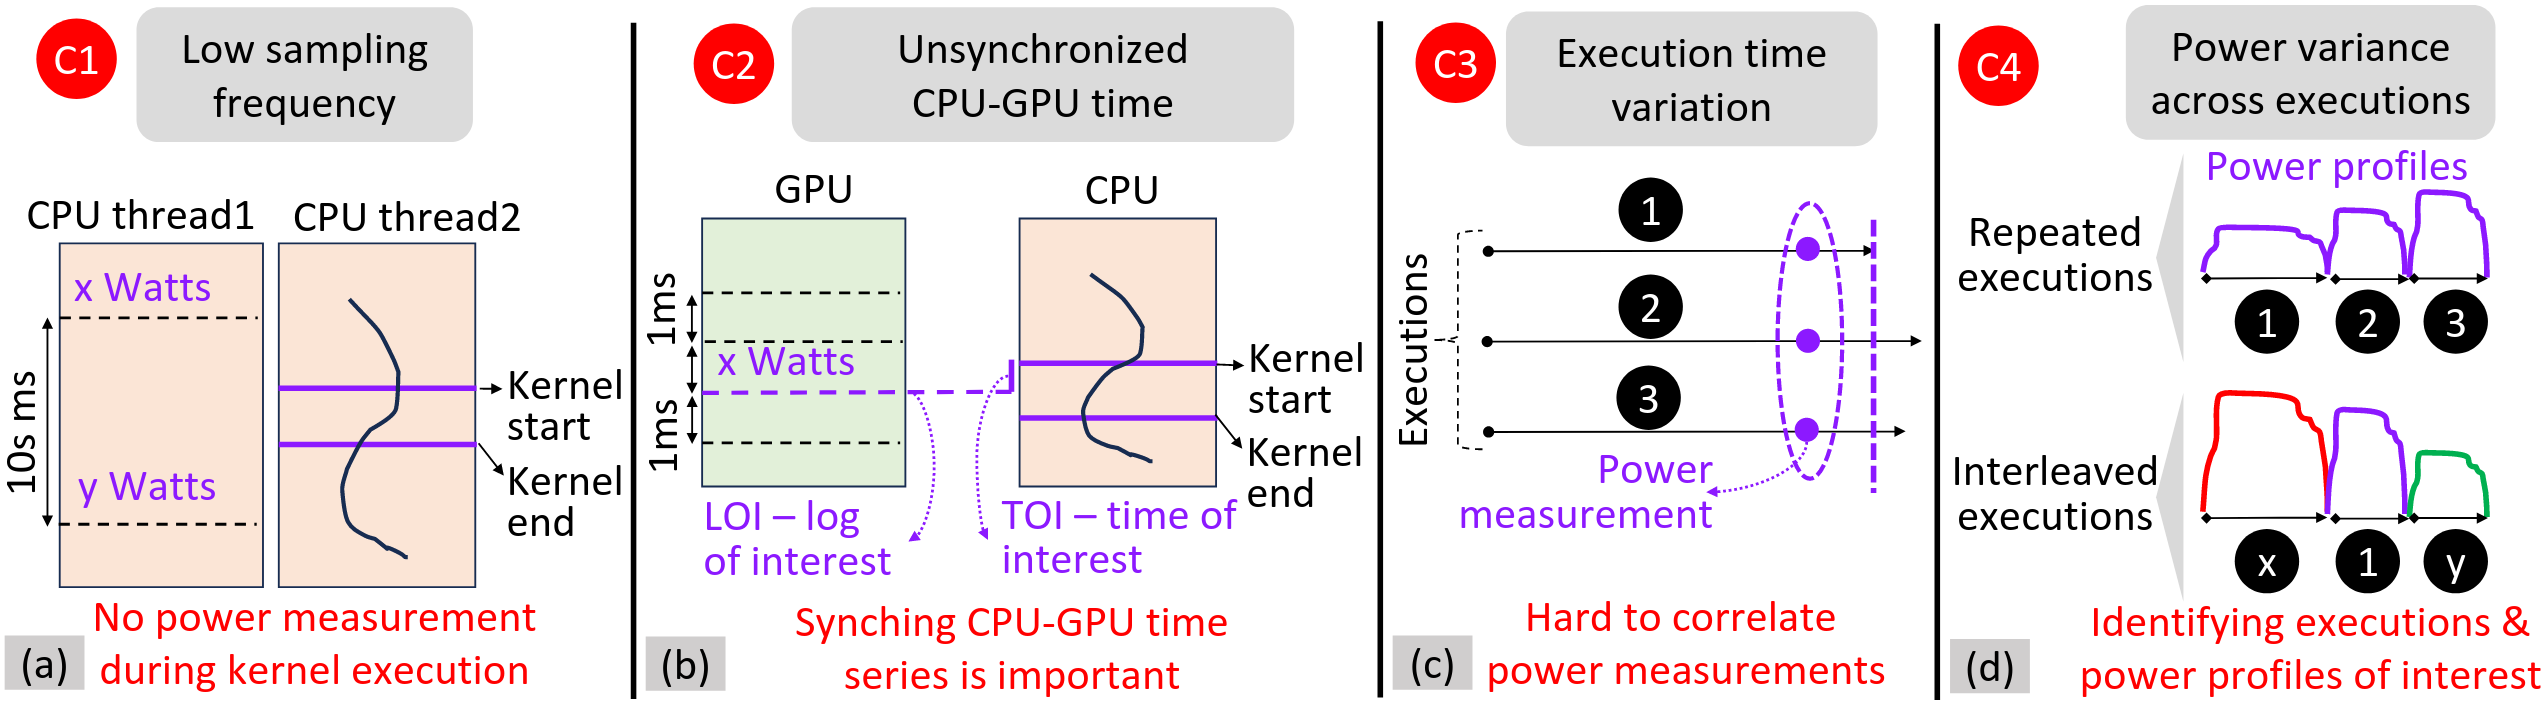
\includegraphics[width=1\textwidth]{Figures/fingrav_challenges.png}
        \caption[Challenges in fine-grain GPU power analysis]{Challenges in fine-grain GPU power analysis}
        \label{fig:fingrav_challenges}
    \end{subfigure}
    \hfill
    \begin{subfigure}{1\textwidth}
        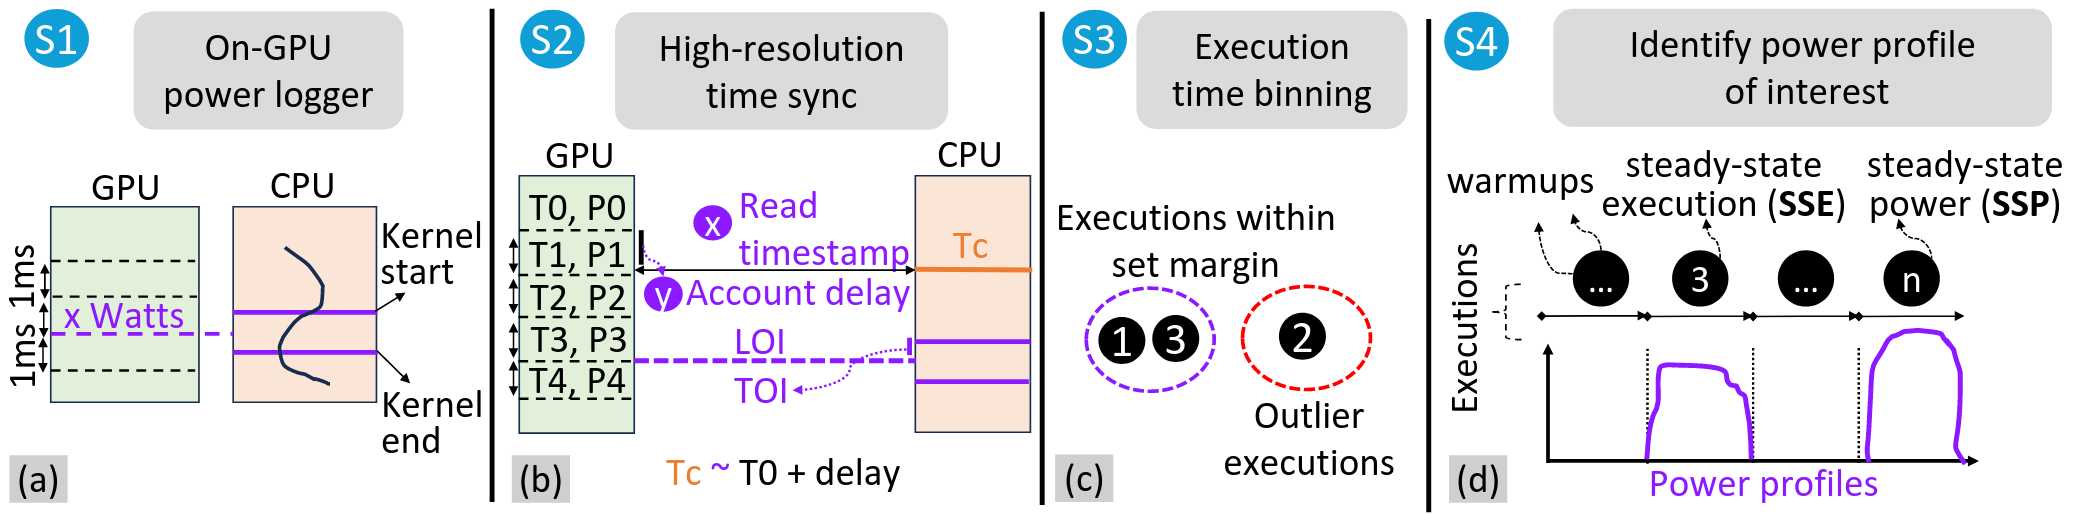
\includegraphics[width=1\textwidth]{Figures/fingrav_solutions.png}
        \caption[FinGraV strategies to adress challenges]{FinGraV strategies to adress challenges}
        \label{fig:fingrav_solutions}
    \end{subfigure}
    \caption[FinGraV GPU power measurement challenges and strategies]{FinGraV GPU power measurement challenges and strategies\parencite{singhania2024methodology}}
    \label{fig:fingrav_challenges_solutions}
\end{figure}

To overcome these challenges, FinGraV introduces several strategies (see figure ~\ref{fig:fingrav_solutions}). 
\begin{itemize}
    \item \textbf{On-GPU Power Logger:} FinGraV leverages a high-resolution (1 ms) power logger, capturing the average of multiple instantaneous power readings.
    \item \textbf{High-Resolution Time Synchronization:} GPU timestamps are read from the CPU side before kernel execution, and synchronization is maintained throughout execution to correlate power samples with kernel events.    
    \item \textbf{Execution Time Binning:} Kernel executions are grouped into "bins" based on empirical runtime ranges, enabling tighter power profiling while discarding outlier runs.    
    \item \textbf{Power Profile Differentiation:} FinGraV distinguishes between Steady-State Execution (SSE) and Steady-State Power (SSP) profiles. SSP represents the stabilized power consumption after initial transients, providing the most accurate depiction of kernel power consumption.
\end{itemize}
The application of FinGraV to bencharmks reveals several critical obervations: Kernel executions differ significantly between initial runs and steady-state, with deviations up to 80\%. Memory-bound kernels and compute-light kernels are found to be highly sensitive to the preceding kernel, impacting their power profile. Furthermore, the authors expose discrepancies in GPU power scaling relative to computational load, particularly for compute-light kernels.

FinGraV introduces promising concepts that could, in theory, enable more granular and accurate GPU power analysis in container-based GPU workloads. Its methodological approach addresses key challenges in sub-millisecond power measurement. However, its current implementation is tightly coupled with the AMD MI300X GPU, relying on hardware-specific logging capabilities that are not universally available. While the underlying concepts may be extendable to other GPUs, achieving this is far from trivial, requiring significant adaptation and low-level access to power metrics that are often proprietary or limited by driver capabilities.

Consequently, FinGraV highlights both the challenges and potential solutions for fine-grained GPU power analysis but falls short of providing a general-purpose framework that could be easily integrated into Kubernetes energy measurement tools. It also underscores the broader issue that GPU energy consumption analysis remains relatively immature, with only vendor-specific tools like nvidia-NVML offering practical (but coarse) power metrics. This illustrates that while the methodology is theoretically sound, practical implementation across diverse GPU architectures remains a significant challenge.

\paragraph{PowerSensor3}
\textit{PowerSensor3}\parencite{van2025powersensor3} is an open-source hardware tool introduced in 2025, designed to provide high-resolution power measurements for GPUs, SoC boards, PCIe devices, SSDs, and FPGAs. Unlike software-based power models or vendor-specific tools such as NVIDIA's NVML, PowerSensor3 achieves significantly higher accuracy and granularity through direct voltage and current measurements at a sampling rate of up to 20 kHz. This fine temporal resolution allows it to capture transient power behaviors that are typically missed by software-based methods, which are constrained by lower sampling frequencies and indirect estimations. As expected for a purpose-built hardware solution, PowerSensor3 outperforms NVML in both precision and the ability to detect rapid changes in power consumption.

A particularly valuable feature of PowerSensor3 is its capability to monitor not only GPUs but also other critical components such as SoC boards, PCIe-connected accelerators, and storage devices like SSDs. For Kubernetes-based energy efficiency analysis, this would provide unprecedented visibility into the power usage of individual containers, extending monitoring beyond the CPU and GPU to the broader spectrum of peripherals that contribute to overall energy consumption. Such granularity could enhance resource scheduling and energy optimization in containerized environments.

However, while its technical benefits are evident, the practical deployment of dedicated hardware sensors like PowerSensor3 at scale remains both complex and expensive. Integrating such devices across large Kubernetes clusters would require substantial investment in hardware and reconfiguration of infrastructure, making wide adoption unlikely outside of specialized research environments. Consequently, PowerSensor3 and other hardware-dependent methods are not considered in the scope of this thesis. Furthermore, the very recent introduction of PowerSensor3 in 2025 highlights the ongoing challenges of accurate energy monitoring through software alone, reflecting the current gap in reliable, scalable, software-based power measurement solutions.

\subsubsection{GPU Limitations in Kubernetes Context}
The analysis of GPU power consumption has revealed promising research efforts aimed at achieving fine-grained power visibility and energy optimization. Tools such as FinGraV and PowerSensor3 demonstrate that significant strides are being made in capturing detailed power metrics with high temporal resolution and sub-component granularity. FinGraV addresses the complexities of short-lived GPU kernel executions through innovative profiling methodologies, while PowerSensor3 delivers hardware-level accuracy for GPUs, SoC boards, and various PCIe-connected peripherals. These solutions underscore the potential for more refined power monitoring in high-performance GPU workloads.

However, the current state of GPU energy consumption measurement presents significant challenges for scalable, container-based energy tracking in Kubernetes environments. Research tools like FinGraV and PowerSensor3, while technically robust, are either hardware-dependent or too tightly coupled to specific architectures (such as AMD's MI300X in the case of FinGraV). Hardware-based solutions like PowerSensor3, though highly accurate, are impractical for widespread deployment due to cost and scalability concerns. Meanwhile, software-based vendor solutions such as NVIDIA's NVML are far more accessible, but suffer from limitations in temporal granularity and measurement accuracy. These tools offer convenient integration and broad support across data center infrastructures but struggle with capturing rapid transients in power consumption, which are crucial for real-time container energy attribution. 

In the context of this thesis, GPU energy consumption is acknowledged as an important yet currently impractical aspect of container energy measurement. The relative immaturity of fine-grained, scalable monitoring solutions for GPUs, combined with the relatively small role of GPUs in Kubernetes clusters, justifies this exclusion. Although the utilization of GPU accelerators in Kubernetes environments is expected to grow, current measurement methods do not yet support the level of precision and scalability required for effective implementation. As such, this thesis will focus on more readily measurable server components, with the understanding that future advancements in GPU power analysis may enable their integration into Kubernetes-based energy efficiency strategies.

\subsection{Storage Devices}
Various sudies have investigated the power consumption of Storage devices. In 2008, Hylick et al\parencite{hylickAnalysisHardDrive2008a} investigated real-time HDD energy consumption and found significant differences in power consumption between standby, idle and active power states. Cho et al\parencite{choDesignTradeoffsSSDs2015} propose various energy estimation models for SSDs after measuring and comparing the energy consumption of different models. The most notabble model-based energy consumption estimation methanisms are presented in section~\ref{sec:model-based_storage_power}

In constrast to CPU or GPU components, storage devices (HDD, DDS or NVMe-drives) cannot make use of physical power sensors. While a BMC-measurement-based solution would technically be feasable, real-world implementation is impractical: While a BMC might me able to measure the power supply to a storage device, it typically is not exposed through IPMI or redfish. Such measurements would further be compllicated by the use of backplane devices, making measurements for individual devices impossible. For these reasons, storage device energy consumption is typically modelled, not measured (see section~\ref{sec:model-based_storage_power}).

While storage devices don't expose any energy-consumption specific metrics, many other related metrics are available (and can be used for modeling approaches):
\begin{itemize}
    \item \texttt{NVMe-cli}\parencite{nvmecli_github} exposes many metrics of NVMe-drives, including the maximum power draw for each power state (including idle power), the number of power states supported, the current power state and temperature, and others.
    \item \texttt{smartctl}\parencite{smartmontools_github} exposes metrics of the \textit{SMART (Self-Monitoring, Analysis and Reporting Technology)}-Functionality implemented in many modern storage drives. While these metrics are vendor-specific, they often include temperature metrics, throughput, and other metrics. Often, HDD speed is exposed. Notably, \textit{SMART} metrics are typically more focussed on lifecycle information such as power-on hours, wear indicators and others.
    \item Many other performance metrics are exposed by various tools such as \texttt{iostat}, \texttt{sar}, \texttt{/proc/diskstats}, and \texttt{blkstat}, such as read/write IOPS, throughput, queue length, latency, utilization, and others. Additional information (such as the interface) is also exposed.
\end{itemize}

\subsection{Network devices and other PCIe devices}

Peripherals like the Network Interace Card (NIC) are almost always connected via PCIe. As such, many cards  support Device power states\parencite{technotes_pci_power_2024} as specified by the PCIe specifications. Notably, not all NICs support all (or any) power states.These device states allow the the server and device to negotiate a power state for the device, which typically means choosing a trade-off between power consumption and wake-up latency. For devices, PCIe specifies the following device states:
\begin{itemize}
    \item D0 state (Fully on)
    \item D1 and D2 states (Intermediate power states)
    \item D3 State (Off State), with the distinction between D3hot and D3cold
\end{itemize}
Unfortunately, device power states are not in any way related to physical power specifications: While a specific power state might be useful for simple deductions (e.g. if a device is idling or active), no power figures can be deduced. In the event that a device's idle or maximum power are known, power states might potentially be used for a first estimation (i.e. an idling device is unlikely to consume its specified maximum power, and vice versa), but since a device's power characteristics cannot reliably estimated (especially beyond just NICs), devices power states cannot be used to reliably estimate device power consumption. An attempt at the estimation of NIC power consumption is covered in section \ref{sec:NIC_modeling}.

\section{Model-based estimation techniques}
In the absence of actual power data, power consumption models can be formulated that map variables (such as CPU or Memory utilization) related to a server's state to its power consumption. 
Due to the strong correlation between CPU uzilization and server power, a great number of models use CPU metrics as the only indicator of server power. Fan et al\parencite{fan2007power} proposed a linear interpolation between idle power and full power, which they further refine into a non-linear form, with a parameter $\gamma$ to be fitted to minimize mean square error. Similar research was done to further reduce error by introducting more complex non-linear models, such as Hsu and Poole\parencite{hsu2011power}, who studied the SPECpower\textunderscore ssj2008-dataset of systems released between December 2007 and August 2010, and suggested the adaptation of two non-linear terms:
\begin{equation}
    P_{\text{server}} = \alpha_0 + \alpha_1 u_{\text{cpu}} + \alpha_2 \left( u_{\text{cpu}} \right)^{\gamma_0} + \alpha_3 \left( 1 - u_{\text{cpu}} \right)^{\gamma_1}
\end{equation}

The division of server power consumption into idle (generally static) and dynamic power (modeled with many different methods thoughought related research) has historically been a popular suggestion\parencite{beloglazovChapter3Taxonomy2011}. Other, broadly similar attempts to model server energy consumption based on only a few variables exist, such as modeling server consumption based on CPU frequency\parencite{elnozahyEnergyEfficientServerClusters2003}.

\subsection{Component-level Power models}

While models like the ones listed above might work well when custom-fitted to specific, multi-purpose servers, they have since been surpassed by the more common approach of modelling server power is to consider it an assembly of its components, such as Song et al\parencite{song2013unified} propose as:
\begin{equation}
    P_{\text{server}} = P_{\text{cpu}} + P_{\text{memory}} + P_{\text{disk}} + P_{\text{NIC}} + C
\end{equation}
where C denotes the server's base power, which includes the power consumption of other components (regarded as static). This approach can easily be extended to include various other components such as GPUs, FPGAs or other connected components.

\subsubsection{Advantages and disadvantages of component-level power models}
A component-based approach to modeling server power consumption offers increased granularity and adaptability across a diverse range of server architectures. Modern data centers deploy heterogeneous hardware configurations optimized for specific workloads, such as CPU-intensive computing nodes, GPU-accelerated servers for machine learning, or memory-rich systems for in-memory databases. These configurations lead to vastly different power distribution profiles across components\parencite{katalEnergyEfficiencyCloud2022}. By modeling the energy consumption of individual components, it becomes possible to reflect these structural differences more accurately. Additionally, such models can reveal energy characteristics that would be obscured in aggregate metrics (for instance, a workload that imposes significant stress on storage devices without engaging the CPU may go undetected in simplistic, CPU-centric models). Finally, component-level analysis enables more precise evaluation of energy optimization techniques: the impact of mechanisms like dynamic voltage and frequency scaling (DVFS) or idle power states can be assessed not just in isolation but in terms of their contribution to overall server efficiency.

Despite offering finer granularity, component-based power modeling faces several inherent challenges. While servers are composed of individual components, they function as tightly integrated systems in which no component operates in isolation. The power consumption of one subsystem often depends on the behavior of others (for example, memory access patterns can influence CPU power states, and I/O activity may trigger CPU wake-ups or increased cache usage). These inter-component interactions are difficult to capture accurately and are frequently overlooked in component-level models\parencite{lin2020taxonomy}, leading to potentially misleading or incomplete estimations. Furthermore, the development of detailed and accurate models for each component is significantly more complex than holistic server-level modeling. Such models often require extensive empirical data, sophisticated estimation techniques, and continuous updates to remain valid across hardware generations. This not only increases the research burden but also demands a higher level of expertise for interpretation and practical application, compared to simpler, utilization-based models.

\subsection{CPU}

Existing CPU power models generally model CPU power as a combination of other, existing power figures. Fan et al\parencite{fan2007power} propose a linear interpolation between idle power and full power based on CPU utilization. Basmadjian et al\parencite{basmadjianMethodologyPredictPower2011} observe that individual cores in a multi-core CPU can be modeled as individual cores, in addition to an overall CPU idle consumption. Non-linear models are also widely adopted, with Lou et al\parencite{LuoEnergyModeling2014} proposing a polynomial model as a univariate function of CPU utilization. Other models include individual CPU components\parencite{basmadjian2012evaluating, sarood2014maximizing} for more fidelity.

While these models may be helpful to examine the dynamics of CPU power consumption in relation to different inputs, they are not helpful in finding CPU power consumption of an unknown CPU, i.e. without previously known idle or maximum power consumption. The existance of a model capable to accurately estimation CPU power consumption based solely on generalizable input factors (such as utilization or frequency) is questionable due to the great variance in architectures and technologies, as well as technological progress. Unsurprisingly, the author of this thesis was not able to find a model to estimate CPU power consumption.

\subsection{Memory}

Many Memory power models were proposed in literature, many of them with an idle and a dynamic component of memory power consumption. While the idle power consumption is generally assumed to be known, dynamic memory power consumption has been modeled to depend on memory usage\parencite{lin2018cloud} or memory accesses\parencite{arroba2014server}, the number of cache misses\parencite{kansal2010virtual}, memory state\parencite{basmadjianMethodologyPredictPower2011}, or other factors. Similar to the CPU models presented in the previous section, these models do not propose generalizable models able to predict memory consumption in situations where idle or maximum memory consumption is not previously known, instead focussing on examining power consumption dynamics. The same objections preventing generalizable CPU models apply to memory models as well, namely great variety, specialization and technological progress. As a result, no model-based approaches exist that are capable of accurately estimating memory power consumption based solely on performance metrics.

\subsection{Storage devices}
\label{sec:model-based_storage_power}

\subsubsection{Generalization-based estimation}
There is an urgent need in the storage industry for research into the area of workload-dependant power estimation\parencite{allaloufStorageModelingPower2009}. Estimating the energy consumption of a storage device is challenging especially due to the great variation between different devices. Some of these model variables can be determined on a running server system (e.g. device type, I/O operation type, access pattern, workload intensity, state and more), while other variables are unknown to the server (e.g. Flash Transition Layer and flash factor, NAND organization, garbage collection, and more). A large storage device market has led to a high variation in devices with sometimes drastically different target uses (e.g. low-latency storage devices, high-concurrency storage devices, low-power storage devices).

Storage controllers further complicate the energy consumption estimation of storage devices by introducing an additional layer of abstraction between the operating system and the physical storage hardware. Their internal operations consume energy independently of the actual read/write workload observed by the host system. This makes it difficult to directly correlate application-level I/O activity with actual device-level power usage. Moreover, in many server configurations, multiple drives are managed behind a single controller, obscuring per-device energy attribution and introducing variability that model-based estimations often cannot accurately capture.

\paragraph{Scope clarification} 
In this thesis, only storage devices physically installed in the server are considered for power estimation. This includes devices such as HDDs, SSDs, and NVMe drives directly attached to the server. Dedicated external storage systems such as Storage Area Networks (SAN) or Network-Attached Storage (NAS) are not within the scope of this analysis. While such systems are important in data center environments, their energy consumption is not attributable at the granularity required for the workload-level estimation pursued in this thesis.

As a result, research into storage device energy consumption measurement that is generally applicable to all devices has been limited. For practical applications, generalizations are often used, such as the following tables~\ref{tab:Storage_power_HDD} to~\ref{tab:Storage_power_NVMe}. While these approximations cannot be used in the context of this thesis, they may serve as an initial guideline.

\begin{table}[H]
    \centering

    \begin{subtable}[t]{\textwidth}
        \centering
        \begin{tabular}{ |c|c|c|c| } 
            \hline
            \textbf{HDD Type} & \textbf{Read/write power (W)} & \textbf{Idle Power (W)} & \textbf{Standby Power (W)} \\
            \Xhline{1.5pt}
            HDD (2.5'' SATA) & 1.5 -- 3.0 & 0.5 -- 1.2 & 0.1 -- 0.3 \\
            \hline
            HDD (3.5'' SATA) & 6 -- 12 & 4 -- 8 & 0.5 -- 2.0 \\
            \hline
            HDD (Enterprise) & 7 -- 15 & 5 -- 10 & 0.5 -- 2.5 \\
            \hline
        \end{tabular}
        \caption[Typical HDD power consumption]{Typical HDD power consumption\parencite{storedbits_hdd}}
        \label{tab:Storage_power_HDD}
    \end{subtable}

    \vspace{1em}

    \begin{subtable}[t]{\textwidth}
        \centering
        \begin{tabular}{ |c|c|c|c| } 
            \hline
            \textbf{HDD Type} & \textbf{Read/write power (W)} & \textbf{Idle Power (W)} & \textbf{Standby Power (W)} \\
            \Xhline{1.5pt}
            5400 RPM HDD & 6 -- 9 & 4 -- 6 & 0.5 -- 1.5 \\
            \hline
            7200 RPM HDD & 8 -- 12 & 6 -- 8 & 0.6 -- 1.8 \\
            \hline
            10,000+ RPM HDD & 10 -- 16 & 8 -- 12 & 1.0 -- 2.5 \\
            \hline
        \end{tabular}
        \caption[Common HDD RPM power consumption]{Common HDD RPM power consumption\parencite{storedbits_hdd}}
        \label{tab:Storage_power_HDD_RPM}
    \end{subtable}

    \vspace{1em}

    \begin{subtable}[t]{\textwidth}
        \centering
        \begin{tabular}{ |c|c|c|c| } 
            \hline
            \textbf{SSD Type} & \textbf{Read Power (W)} & \textbf{Write Power (W)} & \textbf{Idle Power (W)} \\
            \Xhline{1.5pt}
            2.5'' SATA & 4.5 -- 8 & 4.5 -- 8 & 0.30 -- 2 \\
            \hline
            mSATA & 1 -- 5 & 4 -- 8 & 0.20 -- 2 \\
            \hline
            M.2 SATA & 2.5 -- 6 & 4 -- 9 & 0.40 -- 2 \\
            \hline
        \end{tabular}
        \caption[Typical SATA SSD power consumption]{Typical SATA SSD power consumption\parencite{storedbits_ssd}}
        \label{tab:Storage_power_SSD}
    \end{subtable}

    \vspace{1em}

    \begin{subtable}[t]{\textwidth}
        \centering
        \begin{tabular}{ |c|c|c|c| } 
            \hline
            \textbf{NVMe Type} & \textbf{Read/write power (W)} & \textbf{Peak Power (W)} & \textbf{Standby Power (W)} \\
            \Xhline{1.5pt}
            M.2 NVMe PCIe 3.0 & 3 -- 5 & 6 -- 9 & 0.4 -- 1.5 \\
            \hline
            M.2 NVMe PCIe 4.0 & 5 -- 7 & 8 -- 12 & 0.5 -- 2 \\
            \hline
            M.2 NVMe PCIe 5.0 & 8 -- 12 & 12 -- 18 & 0.8 -- 3 \\
            \hline
        \end{tabular}
        \caption[Typical NVMe SSD power consumption]{Typical NVMe SSD power consumption\parencite{storedbits_ssd}}
        \label{tab:Storage_power_NVMe}
    \end{subtable}

    \caption[Power consumption for storage types]{Power consumption for various storage device types.}
    \label{tab:Storage_power_grouped}
\end{table}

Apart from simple estimations like shown in tables~\ref{tab:Storage_power_HDD} to ~\ref{tab:Storage_power_NVMe}, a few works have concentrated on the energy consumption of individual storage devices. In 2015, Cho et al developed Energysim\parencite{choDesignTradeoffsSSDs2015}, an SSD energy modeling framework avancing the understanding of component-level (i.e. the subcomponents of a storage device) energy consumption in storage devices. Its validation against real-world SSD measurements against an Intel X25-M yielded a less than 8\% error. The work underscores the difficulty of modeling storage energy accurately due to high variability across architectures and workloads. Unfortunately, Energysim uses many model parameters such as NAND organization, idle and active current consumption, and as a result cannot reneralized to other storage devices where these are unknown.

In 2014, Li and Long\parencite{liWhichStorageDevice2014} present a workload-aware modeling framework to estimate the energy consumption of storage systems, challenging the assumption that SSDs are inherently more energy-efficient than HDDs. By classifying I/O workloads into capability workloads (performance-driven) and capacity workloads (storage size-driven), they develop mathematical models that account for the number of devices needed, workload execution time, and device power states (active, idle, standby). Their validation, based on empirical measurements using Seagate HDDs and a Samsung SSD, shows that SSDs are generally more efficient for high-performance workloads, while HDDs can outperform SSDs in archival or low-access scenarios,particularly when effective power management (e.g., spin-down) is employed. Unfortunately, similar to the research by Cho et al, the presented models make use of various non-generalizable variables, most notably a devices idle, standby and busy power consumption. In the context of these thesis, these are unknown and the presented model consequently cannot be applied.

\subsubsection{GSPN Modeling for hybrid storage systems (active power states)}
In 2022, Borba et al\parencite{borbaModelingApproachEstimating2022} proposed a number of models based on generalized stochastic Petri nets (GSPN) for performance and energy consumption evaluation for individual and Hybrid (HDD + SSD) storage systems. GSPN is a suitable formalism for storage system design, as, differently from queueing network models (for instance), synchronization, resource sharing, and conflicts are naturally represented. Also, phase approximation technique may be applied for modeling non-exponential activities, and events with zero delays (e.g., workload selection) may adopt immediate transitions. 

The authors propose a single-storage model (either for a single storage device or a hybrid system as a blackbox) and a multiple storage model.

The Hybrid storage power consumption model proposed by Borba is parameterized by I/O type (read/write), access pattern (sequential/random), object size (4KB, 1MB), and thread concurrency. The model explicitely imcorporates power consumption per operation (e.g. random-read-4KB on SSD).

The following notation is adoped:
\begin{itemize}
    \item $E\{\#p\}$ represents the mean value of the inner expression, in which $\#p$ denotes the number of tokens in place.
    \item $W(T)$ represents the firing rate associated with transition $T$.
    \item $\eta : T_{\text{imm}} \rightarrow [0, 1]$ maps each immediate transition ($t \in T_{\text{imm}}$) to a normalized weight. Weights represent the transition firing probablilty in a conflict set.
    \item $pRequests(N)$ denotes the amount of concurrent requests from simultaneous clients (workers)
\end{itemize}

Single-device storage energy consumption is estimated as follows:
\begin{align}
    EP_w = \kappa \cdot (&EP_{w1} \cdot \alpha \cdot \beta 
        + EP_{w2} \cdot (1 - \alpha) \cdot \beta \notag \\
        &+ EP_{w3} \cdot \alpha \cdot (1 - \beta) 
        + EP_{w4} \cdot (1 - \alpha) \cdot (1 - \beta))
\end{align}
\begin{align}
    EP_r = (1 - \kappa) \cdot (&EP_{r5} \cdot \alpha \cdot \beta 
        + EP_{r6} \cdot (1 - \alpha) \cdot \beta \notag \\
        &+ EP_{r7} \cdot \alpha \cdot (1 - \beta) 
        + EP_{r8} \cdot (1 - \alpha) \cdot (1 - \beta))
\end{align}
\begin{equation}
    EC = (EP_w + EP_r) \cdot TH \cdot \text{time}
\end{equation}
where $EP_w$ and $EP_r$ are the mean power consumption for a read ($r$) or write ($w$) operation, which is estimated using the mean power of each workload feature. For instance, $EP_{w1}$ denotes the power of a write operation ($w$) using random access ($\alpha$) and a small object ($\beta$). System throughput (i.e., IOPS) is estimated as $TH = E\{\#p_{\text{Ack}}\} \times W(t_{\text{Communicating}})$.For the single device model, the following weights are taken into account:
$\eta(t_{\text{Write}}) = \kappa$;  
$\eta(t_{\text{Read}}) = 1 - \kappa$;  
$\eta(t_{\text{Random}}) = \alpha$;  
$\eta(t_{\text{Sequential}}) = 1 - \alpha$;  
$\eta(t_{\text{Small}}) = \beta$; and  
$\eta(t_{\text{Large}}) = 1 - \beta$.

The marking of place $pResource (R)$ (for both read or write activity) may denote the adopted technology. For instance, for traditional SSDs (SATA interface), the marking place $pResource$ is 1, as only one operation it the time is carried out. Concerning SSDs-NVMe, $pResource$ assumes the number of threads of concurrently processing I/O requests (generally 8).

The proposed multi-storage model expands the model for multiple devices:
\begin{equation}
    EC_h = \left( \sum_{d=0}^{n} \eta(tForward_d) \cdot EP_d \right) \cdot TH_h \cdot \text{time}
\end{equation}
where the immediate transitions $tForward_d$ denote a request redirection to storage $d$.

\paragraph{Validation}
The model proposed by Borba et al. was validated using controlled experiments with the Fio benchmarking tool, which generated synthetic I/O workloads to measure and correlate storage system performance and energy consumption across varying request sizes, access patterns, and read/write ratios. Model estimates consistently falling within the 95\% confidence intervals of observed system metrics. This statistical consistency indicates that the model's predictions are not significantly different from real-world values, supporting its applicability for performance and energy analysis in large-scale storage systems.

\paragraph{Limitations}
The authors acknowledge that a large number of devices significantly increases modeling complexity due to state space size explosion and recommend simulation as a viable workaround. Additionally, the authors acknowledge their focus on active energy states (not idle, standby states or state transitions), treating them as delays between requests. 

In a running server system, this approach could be adapted to create an accurate and fine-grained energy consumption estimation of a read/write workload on specific storage devices, albeit with limitations:

\begin{itemize}
    \item Instead of needing to be estimated, (device-specific) throughput ($TH$) can be measured.
    \item An intial calibration run is necessary to experimentally determine the respective device-specific variables.
    \item In a multi-storage device server, the resulting state explosion may lead to significan calculation overhead, resulting also in higher energy consumption of the measurement itself.
    \item Instead of modelling transitions to a storage device as a function (as done in $\eta(tForward_d)$), device usage would actively need to be measured, which would essentially transform the multi-storage model into a simple addition of single-storage models. This would drastically reduce the number of total states, making calculations less demanding.
    \item Due to the authors not considering idle and standby-states, a small, constant idle power consumption would need to be added to the model. This is especially important for accurate storage device power consumption modeling on idling or overprovisioned servers.
\end{itemize}

\subsection{Network devices}
\label{sec:NIC_modeling}
Estimating the total power consumption of a network infrastructure requires a clear definition of system boundaries. Since most server clusters operate within larger, interconnected systems, a full assessment of network energy consumption (such as for CO\textsubscript{2} footprint calculations) is generally infeasible. This thesis limits the system boundary to the server itself, considering only internal network components, primarily the Network Interface Card (NIC). While this allows detailed modeling of NIC power usage, it excludes broader network activity, such as inter-node communication in multi-node clusters.

Although the overall energy consumption of a data center network could be estimated by including access, aggregation, and core switches, attributing this consumption to specific workloads remains highly challenging. This chapter therefore focuses on model-based methods for estimating NIC-level power as a proxy for server-side network energy usage.

\subsubsection{NIC power consumption characteristics}
While a lot of research was done to analyze the power consumption of network equipment like switches, routers or gateways, NICs (especially non-wireless NICs) have not received as much attention. While there are several methods that modern NICs employ to save power (e.g. PCIe Link power states and D-states, \textit{Active State Power Management (ASPM)}) or \textit{Energy Efficient Ethernet (EEE)}, there are not widely available mechanisms for fine-grained NIC power consumption estimation. As a consequence, NIC power can only be approximated based on the few available metrics, 

Sohan et al\parencite{sohanCharacterizing10Gbps2010} measured and compared the power consumption of six 10 Gbps and four multiport 1 Gbps NICs at a fine-grained level. While he does not provide a method to estimate NIC energy consumption, and notices great variation in power consumption between different NICs. Unfortunately, it cannot be ruled out that some of the results are cherry-picked: Solarflare-NICs tend to dominate the introduced metics, and a Communication spokesperson is prominently credited with contact information. Regardless, some findings are found irrespective of the NIC manufacturer, and remain consistent with other literature sources\parencite{gough2015energy}. While these findings cannot directly contribute to a potential NIC power consumption estimation approach, they are relevant to understand underlying mechanisms and to assess the relative importance of the NIC compared to other server components.
\begin{itemize}
    \item Idle Power
    \begin{itemize}
        \item The measured NICs show a power consumption of between 5--20W
        \item Link connection status has little effect on idle energy consumption
        \item Physical media influences power consumption: CX4 models have the lowest power consumpttion due to the simple design of the CX4 interconnect. This is followed by Fober models. Finally the Base-T models consume significantly more power due to the signal processing component int he card.
    \end{itemize}
    \item Active Power
    \begin{itemize}
        \item There is very little difference in the power usage of an active NIC compared to an idle one. For all measured NICS, the differenc in power usage was less than 1W.
        \item Throughput performance varied widely, and no correlation between power usage and performance was observed.
        \item Power consumption increases in correlation to the number of ports. 
    \end{itemize}
\end{itemize}

In 2012, Basmadjian et al\parencite{basmadjianCloudComputingIts2012} modelled a NIC by separating NIC power consumption into idle mode and dynamic mode (same as they did for their CPU and RAM models). If $P_{NIC_{idle}}$ is the power of the idle interface and $P_{NIC_{dynamic}}$ is the power when active, the total NIC energy consumption would be given by
\begin{equation}
    E_{NIC} = P_{NIC_{idle}}T_{idle} + P_{NIC_{dynamic}}T_{dynamic}
\end{equation}
where $T_{idle}$ and $T_{dynamic}$ are the total idle and dynamic times, respectively. Consequently, the average power during period $T$ would be given by
\begin{align}
    P_{\text{NIC}} &= \frac{(T - T_{\text{dynamic}}) P_{NIC_{idle}} + P_{NIC_{dynamic}} T_{\text{dynamic}}}{T}\\
                   &= P_{NIC_{idle}} + (P_{NIC_{dynamic}} - P_{NIC_{idle}})\rho
\end{align}
where $\rho=\frac{T_{\text{dynamic}}}{T}$ is the channel utilization. While this formula is only helpful when NIC idle and max power consumption are already known, we can additionally see that the NIC power consumption is assumed to rise linearly with channel utilization.

Arjona Aroca et al\parencite{arjonaarocaMeasurementbasedAnalysisEnergy2014} modeled NIC efficiency based on their previous measurements. They find that NIC efficiencies for both sending and receiving are almost linear with the transfer rate and deduct a linear dependency to the network throughput.

In 2016, De Maio et al\parencite{demaioModellingEnergyConsumption2016} proposed a network energy consumption model for node-to-node transfers in order to estimate the entire energy consumption required for virtual machine migration. Unfortnuately their model does not specifically handle NIC energy consumption, opting for modelling the entire node energy consumption of the node.

Another approach is presented by Dargie and Wen\parencite{dargieProbabilisticModelEstimating2013} in 2013, who use stochastic modelling to examine the relationship between the utilization of a NIC and its power consumption, expressing these quantities as random variables or processes. They use curve fitting to determine the relationship between utilization and measured energy consumption of their specific NIC, after creating a data set using a SPECpower benchmark. They assume a uniformly distributed bandwidth utilization in the interval [0,125] MBps. Interestingly, their model shows only a slight effect of utilization on the predicted power consumption, mirroring the findings of Sohan et al.

The most recent NIC power model was proposed by Baneshi et al\parencite{baneshiAnalyzingPerApplicationEnergy2024} in 2024, analyze per-application energy consumption. The authors cite that NIC idle power consumption may contribute up to 90\% of the total NIC energy consumption. They propose the following model for per-application NIC power consumption:
\begin{equation}
    E_{\text{active}} = \sum_{i} \left( BW_i \cdot T_{\text{interval}} \cdot \frac{P_{\text{max}} - P_{\text{idle}}}{BW_{\text{aggregated}}} \right)
\end{equation}
\begin{equation}
    E_{\text{idle}} = \sum_{i} \left( BW_i \cdot T_{\text{interval}} \cdot \frac{P_{\text{idle}}}{BW_{\text{used}}} \right)
\end{equation}
where $BW_i$ is the bandwidth of application i, $BW_{\text{aggregated}}$ is the aggregate bandwith of both the uplink and downlink of the NIC, and $BW_{\text{used}}$ is the used bandwidth of links (uplinks, downlinks or both). The authors combine these formulae with power figures of their specific use case (Total network power consumption in a fog computing scenario), which unfortunately are not applicable in the context of this thesis. Regardless, while these formulae cannot be used to estimate the maximum and idle NIC power, they can be applied irrespective of server specifications in the event that idle and maximum power NIC power consumption are known.

In contrast to the formulae presented by Basmadjian and Arjona Aroca, the formulae not only account for time intervals, but also bandwidth used. As a result, the formulae presented by Baneshi et al represent the current best approach to estimate NIC power consumption, even though this estimation still requires an initial guess of the idle and maximum power consumption. The author of this thesis is not aware of a more detailed formuala currently available. A generalizable formula for estimating overall NIC power consumption is unlikely to exist due to the vast variety of NICs, and the great differences between manufacturers (as found by Sohan et al). 

\subsection{Other devices}
While much of the research on server energy consumption focuses on primary components such as the CPU, memory, storage, and network interfaces, a complete energy model must also account for additional hardware subsystems. These include the motherboard, power supply unit (PSU), system fans, and potentially other auxiliary devices. Though their individual energy consumption may appear minor compared to high-performance components, they collectively contribute a non-negligible share to the overall server power draw.

Despite their importance, these secondary components have received limited attention in energy modeling literature. In most cases, they are either omitted or treated as part of the residual power not attributable to the main computational subsystems.

The motherboard, for instance, includes voltage regulators, chipset logic, and peripheral interfaces. While these components may not be individually monitored, the Baseboard Management Controller (BMC) (see section ~\ref{sec:BMC_devices})may expose aggregated power telemetry via vendor-specific sensors or interfaces like IPMI or Redfish. However, this level of detail varies greatly across hardware platforms and is seldom fine-grained enough for component-level attribution.
\subsubsection{PSU}
The power supply unit (PSU) is another often-overlooked consumer. When modeling the power usage of a PSU itself (distinct from the power it delivers to other components), the key factor is its conversion efficiency. PSUs consume more power than they deliver due to losses during AC–DC transformation and voltage regulation. According to Basmadjian et al. \parencite{basmadjianCloudComputingIts2012}, the power consumed by the PSU can be approximated for various scenarios:
If the monitoring system provides information at the PSU level, its power consumption is given by
\begin{equation}
    P_{PSU} = \frac{measuredPower \cdot (100 - e)}{100}
\end{equation}
where $e$ is the efficiency of the PSU.

If the monitoring system proves information at the server level, the power consumption of any of the $n$ PSU is given by the following formuala, assuming that measured power is evenly distributed among PSUs:
\begin{equation}
    P_{PSU} = \frac{\frac{measuredPower}{n} \cdot (100 - e)}{100}
\end{equation}

If the monitoring system does not provide PSU power consumption, it can be deduced by
\begin{equation}
    P_{PSU} = \frac{P_{Mainboard} + P_{Fans}}{n \cdot e} \cdot 100 - \frac{P_{Mainboard} + P_{Fans}}{n}
\end{equation}

\subsubsection{Fans}
Cooling systems, particularly fans, also represent a meaningful share of the total energy budget. Most servers employ multiple fans controlled via Pulse-Width Modulation (PWM). While the BMC or operating system tools (e.g. \texttt{lm-sensors}) often report fan RPM or PWM duty cycle, actual fan power consumption is rarely exposed directly. Furthermore, RPM alone is insufficient to estimate power accurately, as fan power depends on physical factors such as the fan diameter, pressure increase or air flow delived\parencite{basmadjianCloudComputingIts2012}:
\begin{equation}
\label{for:fanpower}
    P_{Fan} = d_p \cdot q = \frac{F}{A} \cdot \frac{V}{t} = \frac{F \cdot d}{t}
\end{equation}
where $p_d$ denotes total pressure increase of the fan (Pa or N/m\textsuperscript{2}), $q$ denotes the air volume flow (m\textsuperscript{3}/s), $F$ denotes force (N), $A$ denotes fan area (m\textsuperscript{2}), $V$ denotes volume (m\textsuperscript{3}), and $t$ denotes time (seconds).

Based on observations, $F$ is proportional with to the sqare of $RPM$. This can be combined with formula ~\ref{for:fanpower}:
\begin{equation}
    P_{Fan} = \frac{c \cdot RPM\textsuperscript{2} \cdot d}{3600}
\end{equation}
where for each individual fan, $c = \frac{3600 \cdot P_{Max}}{RPM_{Max}\textsuperscript{2} \cdot d}$ remains constant.

Unfortunately, with the wide variety of fans in servers (especially with fan size restrictions due to server heights), these formulae are only helpful when paired with more detailed information on fan characteristics like Maximum RPM and Power. While these can more reasonably be assumed, this remains a rough estimation at best.

\subsubsection{Attribution of secondary component power consumption to individual workloads}
Despite these measurement limitations, estimating the energy consumption of secondary components is often less critical for attributing energy to workloads. This is because components like fans, mainboards, and PSUs primarily support the operation of primary subsystems. Their power consumption scales with the activity level of CPU, memory, disk, and networking devices: more computation leads to higher heat dissipation, increased power delivery, and thus greater fan and PSU activity.

Consequently, if the total server power consumption is known—for example, via wall power monitoring or BMC/Redfish readings—the residual power (i.e., total power minus the sum of measured CPU, RAM, disk, and network power) can be reasonably attributed to power delivery and thermal management subsystems. This residual can then be proportionally distributed among active workloads based on the power consumption of the primary components they utilize. In this context, fine-grained modeling of secondary components becomes unnecessary for workload attribution, as their energy use correlates closely with that of the primary subsystems they support.

\subsection{Issues with model-based power estimation techniques}
This thesis pursues two inherently conflicting objectives: achieving high-resolution, accurate energy consumption measurements while simultaneously developing a solution that remains broadly applicable across heterogeneous server environments without requiring extensive manual calibration, or the manual input of complex device-specific information. Striking a balance between these goals is particularly challenging in the context of model-based energy estimation for devices that do not expose power telemtry data: Due to the wide variability among devices for a variety of factors, energy consumption models must necessarily abstract away much of the underlying complexity. Developing a model that is simultaneously fine-grained, highly accurate, and universally applicable across different technologies is, in practice, an unattainable goal.

As a result, any model integrated into a general-purpose energy estimation framework must err on the side of relative simplicity to preserve generality. While this approach diminishes the precision of device-specific energy attribution, it remains valuable for broader optimization tasks. For instance, autoscaling mechanisms, load balancers, and schedulers can still benefit significantly from approximate energy profiles. Likewise, cluster administrators aiming to improve energy efficiency holistically, or developers seeking to optimize their workloads, can gain useful directional insights even from coarse-grained models.

However, this simplicity imposes significant limitations for use cases that require device-specific energy optimization. General-purpose models are ill-suited for evaluating the energy efficiency of different device types, testing firmware-level adjustments, or validating the impact of power-saving features such as low-power states. In such scenarios, the model’s abstraction may not just be insufficient, but actively misleading.

In the context of this thesis, this limitation is considered acceptable. The overarching objective is to facilitate scalable and portable energy estimation mechanisms for containerized environments, not to provide a diagnostic tool for hardware-level energy analysis. Nonetheless, this constraint should be kept in mind when interpreting the results and assessing their suitability for device-centric evaluation tasks.

\section{Power Modeling based on Machine Learning Algorithms}

In a taxonomy of power consumption modeling approaches, Lin et al\parencite{lin2020taxonomy} analyze various machine learning-based power models in current literature, categorizing them into supervised, unsupervised, and reinforcement learning. A detailed reiteration of this taxonomy (as well as a methodological overview of machine learning and neural networks) is omitted here.

In the context of this thesis, machine learning-based approaches are not considered for the following reasons:
\begin{itemize}
\item The author was unable to identify a promising and reliable approach that is sufficiently generalizable to function across a wide range of server configurations. Likewise, no component-level models were found that met these criteria. While it is certainly possible to train machine learning models to estimate energy consumption for specific server setups with high accuracy, the aim of this thesis is to provide generalizable estimation methods applicable to varied systems.
\item Machine learning fundamentally relies on large datasets that are both highly accurate and granular, ideally matching the quality expectations of the resulting model. As discussed in previous sections, such high-quality training data is rarely available in the domain of fine-grained power measurement. When such datasets do exist, they typically reflect highly specific hardware and workload configurations, making them unsuitable for generalization. Although it would be theoretically possible to generate a large dataset by systematically benchmarking thousands of CPUs, memory modules, GPUs, storage, and network devices across millions of configurations, such an undertaking is not practically feasible. Furthermore, any such dataset would require ongoing expansion to remain representative of new hardware generations.
\item Finally, many of the technical implementation details underlying key telemetry features remain proprietary or undocumented. A notable example is the RAPL interface, whose internal workings are not publicly disclosed. At the same time, existing RAPL metrics already offer abstracted energy readings suitable for direct integration into power estimation tools, eliminating the need for an intermediate machine learning-based step.
\end{itemize}

In theory, machine learning-based power estimation models hold significant promise and may one day be realized. Such models could leverage complex, nonlinear relationships between hardware components and workloads—relationships that are inherently difficult or even impossible to capture through traditional analytical models. The predictive and adaptive capabilities of machine learning offer the potential for highly accurate, fine-grained estimations across a broad range of configurations. However, as of today, the development of such a comprehensive and generalizable model remains out of reach. Realizing this vision would require extensive collaboration between original equipment manufacturers, cloud providers, data center operators, and research institutions to generate, standardize, and share high-quality telemetry data across diverse hardware and workload scenarios. Given the role of cloud computing in the current economic landscape, where proprietary knowledge and performance optimization constitute a competitive advantage at the corporate, national, and geopolitical levels, such broad cooperation appears unlikely. Consequently, machine learning remains a promising but currently impractical direction for universal server power modeling.



\section{Container energy estimation based on hardware power estimation}
% see lin et al


\section{Component-specific summaries}
\label{sec:component_specific_summaries}

see Lin et al for overview -> instruments / dedicated aquisition system / software monitoring and calculation / simulation

\subsection{CPU}

\subsection{Memory}

\subsection{GPU}

\subsection{Storage devices}

\subsection{Network devices}